% !TEX root =../../cursus 5ICWE.tex
\chapter{De Coulombkracht}
\todo{hoofdstuk maken}
% ----------------------------------------------------------------------
%          inleiding hoofdstuk
% ----------------------------------------------------------------------
De elektromagnetische kracht tussen geladen deeltjes is één van de vier fundamentele natuurkrachten. In dit hoofdstuk onderzoeken we eerst de basiseigenschappen van elektrische lading en de krachten die erop inwerken. Vervolgens bekijken we hoe objecten een lading kunnen krijgen, onder andere met behulp van de \emph{tribo-elektrische reeks}.

Daarna verdiepen we ons in de \emph{wet van Coulomb}, die zowel de grootte als de richting van de kracht tussen geladen deeltjes beschrijft. Je leert hoe je deze kracht kunt berekenen in uiteenlopende situaties, en we sluiten af met enkele praktische toepassingen.

Dit geheel behoort tot de \emph{elektrostatica}: het gedrag van stilstaande ladingen. In latere hoofdstukken bestuderen we ook bewegende ladingen en de verschijnselen die daarbij horen.
\begin{definitie}
\emph{Elektrostatica} is het deel van de fysica dat het gedrag en de interacties van elektrische ladingen in rust en de krachtwerking er tussen bestudeert.
\end{definitie}
% ----------------------------------------------------------------------
%          lading
% ----------------------------------------------------------------------
\section{Eigenschappen van Elektrische Ladingen}
Er zijn simpele experimentjes om aan te tonen dat er elektrische krachten zijn. Zo gaan je haren rechtstaan als je met een ballon over je haar wrijft. Of het aantrekken van papieren snippers met een wollen trui waarover je hebt gewreven.
% -------------------------
%yt video naar demonstratie met papier snippers
\begin{marginfigure}
	\begin{center}
		\qrcode[hyperlink,height=0.85in]{https://youtu.be/Glifj-apltU}
	\end{center}
	\vspace*{-5mm}
	\caption*{{\scriptsize  Link naar video met het aantrekken van papiersnippers.}}
\end{marginfigure}
% ---------------------------

%--------------------------
% afbeelding buisjes
\begin{figure}[htbp]
\captionsetup{width=0.85\textwidth}
\begin{center}

\includegraphics[width=0.8\textwidth]{hoofdstukken/Elektromagnetisme/buisjes.jpg}
\caption{(a) Een negatief geladen rubberen staaf die aan een draad hangt, wordt aangetrokken door een positief geladen glazen staaf. (b) Een negatief geladen rubberen staaf wordt afgestoten door een andere negatief geladen rubberen staaf.}
\label{fig:buisjes}
\end{center}
\end{figure}
% --------------------------

% -------------------------
%	eigenschappen van ladingen en soorten ladingen
% -------------------------------

In een reeks van simpele experimenten kan er aangetoond worden dat er maar twee soorten ladingen bestaan en is als gevolg hiervan het deeltjes model uitgebreid:
\begin{itemize}
 	\item er bestaan twee soorten ladingen: \textcolor{red}{\textbf{positieve}} ladingen (+) en \textcolor{blue}{\textbf{negatieve}} ladingen (-). \mn{Conventie voor de kleuren: \textcolor{red}{rood} voor \textcolor{red}{positieve} lading en \textcolor{blue}{blauw}/zwart voor \textcolor{blue}{negatieve} ladingen}
	\item de kracht dat ladingen op elkaar uitoefenen is de elektrische kracht. \textbf{Gelijksoortige ladingen stoten elkaar af} en \textbf{verschillende soorten ladingen trekken elkaar aan}.
	\item \textbf{lading blijft behouden}. Lading kan niet vernietigd of gemaakt worden, enkel uitgewisseld.
	\end{itemize}
	\begin{wet}
	\textbf{Behoud van lading}\\ De totale elektrische lading in een gesloten systeem blijft altijd gelijk. Met andere woorden: lading kan niet uit het niets ontstaan of zomaar verdwijnen. Ze kan enkel worden verplaatst van het ene voorwerp naar het andere. Wanneer een voorwerp elektronen verliest, neemt een ander voorwerp ze op, zodat de totale hoeveelheid lading onveranderd blijft.
	\end{wet}
	\begin{itemize}
	\item lading is \textbf{gekwantiseerd}\mn{ Gekwantiseerd betekent dat een bepaalde grootheid niet willekeurig elke waarde kan aannemen, maar enkel specifieke, discrete waarden. Deze waarden wordt \textit{e} genoemd. $\mathit{e}=1,6\cdot 10^{-19}\unit{\coulomb}$. De huidige theorieën laten wel breuken van deze lading toe voor quarks, al zijn \textit{vrije} quarks nog nooit gevonden. Meer hier over in hoofdstuk~\ref{hoofdstuk: Deeltjes Fysica}} 
\end{itemize}
\begin{theorie}
De \textbf{ladingshoeveelheid}, of ook wel elektrische lading, stellen we voor door \textbf{Q}. De eenheid van ladingshoeveelheid is de coulomb (C).
\end{theorie}


Lange tijd dacht men dat lading en materie twee gescheiden domeinen van de wetenschap waren. Onderzoek heeft echter aangetoond dat lading voorkomt in de deeltjes waaruit ook materie is opgebouwd. Materie bestaat uit atomen, en atomen bestaan uit protonen, neutronen en elektronen. Meer informatie over de bouwstenen van alle deeltjes volgt in een later hoofdstuk: hoofdstuk~\ref{hoofdstuk: De Atoomkern}.

% TABEL MET GEGEVENS NUCLEONEN
\begin{table}[h!]
\caption{Lading en Massa van de Proton, Neutron en het Elektron}
\centering
\begin{tabular}{@{}lcr@{}}
	\toprule
	deeltje & lading (C) & massa (kg)\\
	\midrule
	\textcolor{red}{proton} & $+1,60\cdot 10^{-19}$ & $1,673\cdot 10^{-27}$ \\
	neutron & 0 & $1,675\cdot 10^{-27}$ \\
	\textcolor{blue}{elektron} & $-1,60\cdot 10^{-19}$ & $9,109\cdot 10^{-31}$ \\
	\bottomrule
\end{tabular}
\vspace{2mm}
	\begin{opm}
		De ladingshoeveelheid is vanbuiten te kennen, de massa van de deeltjes niet. Coulomb is een grote eenheid, dus vaak zal er gebruik worden gemaakt van voorvoegsels zoals mili, micro en nano. Zie appendix~\ref{hoofdstuk: Standaardvorm}.
	\end{opm}
\end{table}
% ----------
%	Tribo-elektrische reeks
% -----------------------

\marginnote{\small Een atoom bestaat uit een kern van protonen en neutronen in het midden, omgeven door een elektronenwolk. Alleen de elektronen kunnen aan een atoom worden toegevoegd of ervan worden onttrokken; protonen worden nooit uitgewisseld.}

Omdat alle materie is opgebouwd uit atomen, en atomen op hun beurt uit elektronen, protonen en neutronen bestaan, bevat elke stof geladen deeltjes. In de meeste gevallen bevatten atomen evenveel protonen als elektronen. Wanneer een stof evenveel positieve als negatieve ladingen bevat, is ze elektrisch neutraal.

Een stof kan enkel een lading \textit{krijgen} wanneer er ladingen worden uitgewisseld. Een stof wordt negatief geladen wanneer ze extra elektronen opneemt, en positief geladen wanneer ze elektronen afstaat.

%------------
% QUIZ 1: AFSTOTEN OF AANTREKKEN
\begin{quiz}\label{q:aantrekken of afstoten}
	Welke van de volgende uitspraken is correct? (a) Twee positieve ladingen trekken elkaar aan. (b) Twee negatieve ladingen stoten elkaar af. (c) Een positieve en een negatieve lading stoten elkaar af. (d) Twee ladingen oefenen geen kracht op elkaar uit.
\end{quiz}
%---------------
%---------------------------------------------------------
%QUIZ 2: EIGENSCHAPPEN VAN LADINGEN
\vspace{2mm}
\begin{quiz}\label{q:eigenschappen ladingen} 
Drie objecten worden telkens per twee in elkaars buurt gebracht. Wanneer objecten A en B samenkomen, stoten ze elkaar af. Wanneer objecten B en C samenkomen, stoten ook zij elkaar af. Welke van de volgende uitspraken is/zijn correct? (a) Objecten A en C hebben een lading met hetzelfde teken. (b) Objecten A en C hebben ladingen met een verschillend teken. (c) Alle drie de objecten hebben een lading met hetzelfde teken. (d) Eén object is netraal geladen. (e) Er zijn nog extra experimenten nodig om het teken van de ladingen te bepalen.
\end{quiz}
%------------------------------------------------------------

%Definitie tribo-elektisch effect
\begin{definitie}
	Het \textbf{tribo-elektrisch effect} is een soort contactelektrificatie waarbij de materialen die met elkaar in contact komen tijdens het wrijven elektrische lading uitwisselen en zo elektrisch opgeladen worden.
\end{definitie}

%\newpage %om de reeks te laten kloppen op papier
\begin{margintable}
	\caption{Tribe-elektrische reeks}
		\begin{tabularx}{\marginparwidth}{@{}r@{}}
			\toprule
			Meest positief geladen\\
			\midrule
			Droge huid\\
			konijnenvel\\
			glas\\
			haar\\
			nylon\\
			wol\\
			lood\\
			zijde\\
			aluminium\\
			papier\\
			katoen\\
			staal\\
			hout\\
			luciet
			amber\\
			plexiglas\\
			rubber\\
			nikkel, koper\\
			polyester\\
			vinyl (pvc)\\
			teflon\\
			\midrule
			Meest negatief geladen\\
			\bottomrule
			\addlinespace[3mm]
		\end{tabularx}
		\label{tabel: tribo-elektrische reeks}
\end{margintable}
Wanneer je een materiaal dat hoger in de tribo-elektrische reeks staat wrijft met een materiaal dat lager in de reeks staat, zal het hoger geplaatste materiaal elektronen afstaan en daardoor positief geladen worden. Het lager geplaatste materiaal neemt deze elektronen op en wordt negatief geladen.
%---voorbeeld: 


%------------------------------------------------------
%QUIZ 3: TRIBO_ELEKTRISHCE REEKS
\vspace{2mm}
\begin{quiz}\label{q:tribo-elektrische reeks} 
Je wrijft met rubber op een PVC buis. Wat kan je zeggen over de lading van beide stoffen? Maak gebruik van tabel~\ref{tabel: tribo-elektrische reeks}. (a) Beide stoffen worden negatief geladen na het wrijven. (b) Rubber wordt positief geladen en PVC negatief geladen. (c) Rubber wordt negatief geladen en PVC positief geladen. (d) Beide stoffen worden positief geladen. (e) Met deze tabel kan je de soort lading niet bepalen. (f) Rubber en PVC kunnen niet tegen elkaar gewreven worden om lading uit te wisselen.
\end{quiz}
%------------------------------------------------------

% ----------------------
% laden via inductie
% -----------------------
\section{Objecten Laden via Inductie}
\subsection{Geleiders, Isolatoren en Halfgeleiders}
\begin{marginfigure}
		\begin{center}
		\begin{subfigure}{.2\textwidth}
			\centering
			\begin{circuitikz}%
				\draw (0,0) node[ ground ] {};%(2,0); 
			\end{circuitikz}%
		\caption{}
		\label{fig:symbool aarding}
	\end{subfigure}%
	\begin{subfigure}{.5\textwidth}
		\centering
		\includegraphics[width=.95\textwidth]{hoofdstukken/elektromagnetisme/aarding kabels.jpeg}
		\caption{}
		\label{fig:kleur aarding}
	\end{subfigure}
		\end{center}
		\caption{(a) Symbool voor aarding. (b) kleur van aarding in kabels is geel+groen.}
		\label{f:aarding}
\end{marginfigure}



\begin{her}
	Aarding is de benaming als je iets met de aarde aansluit.	Hierdoor kan een teveel van elektronen gecompenseerd worden door elektronen naar de aarde te sturen, of kan bij een tekort van elektronen er elektronen van de aarde onttrokken worden.
\end{her}
% SUBSECTION: geleiders
\subsubsection{Geleiders}
De meeste metalen zijn goede geleiders. In de chemie heb je al kennisgemaakt met het metaalrooster. Metaalatomen bezitten elektronen die gemakkelijk loskomen van het atoom: de zogenaamde valentie-elektronen. Deze elektronen bewegen ‘vrij’ door het rooster van positieve metaalionen.

De vrije elektronen botsen voortdurend met de roosterionen, zie figuur~\ref{fig:metaal}, waardoor hun bewegingsrichting en bewegingszin steeds veranderen. Hun gemiddelde snelheid is daardoor nul. Toch kunnen de vrije elektronen zich binnen het metaal verplaatsen, en ook van het ene metaal naar het andere wanneer beide in contact staan. Dankzij het grote aantal vrije elektronen zijn metalen uitstekende geleiders.
% --------------------
% beweging elektronen geleider en isolator
\begin{marginfigure}
	\begin{center}
		\qrcode[hyperlink,height=0.85in]{https://youtu.be/gm5cepGTDKo}
	\end{center}
	\vspace*{-5mm}
	\caption*{\scriptsize Link naar video met de beweging van elektronen van geleiders en isolatoren.}
\end{marginfigure}
% -----------------------------------

%-----------------------------
%	afbeelding elektronen rond geleider
\begin{figure}[H]
\captionsetup{width=0.85\textwidth}
	\centering
	\begin{subfigure}{.5\textwidth}
		\centering
		
\includegraphics[width=.95\textwidth]{hoofdstukken/elektromagnetisme/metaal1.png}
		\caption{}
		\label{fig:metaal1}
	\end{subfigure}%
	\begin{subfigure}{.5\textwidth}
		\centering
		
\includegraphics[width=.95\textwidth]{hoofdstukken/elektromagnetisme/metaal2.png}
		\caption{}
		\label{fig:metaal2}
	\end{subfigure}
	\caption{(a) De valentie-elektronen komen los van de atomen en kunnen vrij bewegen tussen de metaalionen. De overige elektronen blijven gebonden aan de atoomkern. (b) De ‘vrije’ elektronen veranderen voortdurend van richting en zin door botsingen met de roosterionen.}
	\label{fig:metaal}
\end{figure}
% ------------------------------
% ---------------------
%	geleiders
% -------------------
\begin{theorie}
Een metaal in vaste toestand bevat vrije (negatieve) elektronen en vaste (positieve) roosterionen.
\end{theorie}

\begin{figure}[H]
	\marginnote{Er zouden ook een elektronen op de metalen staaf gezet kunnen worden.}
	\captionsetup{width=0.85\textwidth}
	\centering
	\begin{subfigure}{.25\textwidth}
		\centering
		\includegraphics[width=\textwidth]{hoofdstukken/elektromagnetisme/metalen staaf 1.jpeg}
		\caption{}
		\label{fig:metalen staaf 1}
	\end{subfigure}%
	\begin{subfigure}{.25\textwidth}
		\centering
		\includegraphics[width=\textwidth]{hoofdstukken/elektromagnetisme/metalen staaf 2.jpeg}
		\caption{}
		\label{fig:metalen staaf 2}
	\end{subfigure}%
	\begin{subfigure}{.25\textwidth}
		\centering
		\includegraphics[width=\textwidth]{hoofdstukken/elektromagnetisme/metalen staaf 3.jpeg}
		\caption{}
		\label{fig:metalen staaf 3}
	\end{subfigure}%	
	\begin{subfigure}{.25\textwidth}
		\centering
		\includegraphics[width=\textwidth]{hoofdstukken/elektromagnetisme/metalen staaf 4.jpeg}
		\caption{}
		\label{fig:metalen staaf 4}
	\end{subfigure}%
	\caption{(a) Een neutrale metalen staaf. Het bevat even veel positieve als negatieve ladingen. (b) Wanneer er elektronen aan de metalen staaf worden onttrokken, krijgt de staaf een positieve lading. Omdat metaal een goede geleider is, wordt het tekort aan elektronen gelijkmatig over de hele staaf verdeeld. (c) De positief geladen staaf wordt verbonden met de aarding. (d) Via de aarding kunnen nieuwe elektronen worden aangevoerd. Omdat metaal een goede geleider is, zullen deze elektronen zich gelijkmatig over de staaf verdelen. }
	\label{fig:metalen staaf}
\end{figure}

Een metalen staaf kan positief geladen worden door elektronen af te geven, zie tekening~\ref{fig:metalen staaf 2}. Vermits de elektronen zich vrij kunnen bewegen, gaat het tekort aan elektronen zich gelijkmatig verspreiden over het hele oppervlak aan de buitenkant van de staaf en zo ver mogelijk van elkaar. Voor een positief geladen staaf is er op de buitenkant van de staaf een tekort aan vrije elektronen. 

Ga je de staaf met de aarde verbinden door middel van een isolator dan gebeurt er niets, zie tekening~\ref{fig:metalen staaf 3}. Verbind je de staaf met de aarde door middel van een geleider dan gaan er via de aarding elektronen van de aarde naar de staaf en wordt de staaf terug neutraal, zie tekening~\ref{fig:metalen staaf 4}.

Een metalen staaf kan negatief geladen worden door elektronen op te nemen. Omdat de elektronen zich vrij kunnen bewegen, verspreiden ze zich gelijkmatig over het hele oppervlak aan de buitenkant van de staaf, zo ver mogelijk van elkaar. Voor een negatief geladen staaf betekent dit dat er een overschot aan vrije elektronen aanwezig is aan de buitenzijde.

\begin{marginfigure}
	\begin{center}
		\qrcode[hyperlink,height=0.85in]{https://youtu.be/bfw8XaQExqc}
	\end{center}
	\vspace*{-5mm}
	\caption*{\scriptsize Link naar video waar ladingen naderen bij een geleider.}
\end{marginfigure}

\begin{opm}
Positieve roosterionen kunnen niet verplaatsen: zij hebben een vaste positie in het metaalrooster.
\end{opm}
% --------------
%	Influentie
% ---------------
\begin{theorie}
	\textbf{Influentie of elektrostatische inductie} is het scheiden van een lading in een geleider wanneer die in de nabijheid komt van een geladen voorwerp.
	Een geaarde geleider wordt geladen wanneer een geladen voorwerp in de buurt wordt gebracht. De lading van de geleider zal steeds tegengesteld zijn aan de lading van het voorwerp.
\end{theorie}

% ----------------------
%	SUBSECTION: Isolator
% ----------------------
\subsubsection{Isolatoren}

Atomen uit groep 15, 16 of 17 van het periodiek systeem staan geen elektronen af. In een vaste stof vormen ze bindingen met andere atomen en gedragen ze zich als isolatoren. Voor wrijvingsproeven gebruik je daarom isolatoren: de aangebrachte ladingen verplaatsen zich niet. De elektronen blijven zitten waar ze zijn aangebracht (zie tekening~\ref{fig:isolator staaf 2}), zelfs wanneer je een geleidende verbinding maakt met de aarde (zie tekening~\ref{fig:isolator staaf 3}). De lading verdwijnt enkel door contact met een tegengesteld geladen voorwerp of door interactie met moleculen in de lucht (ionisatie).


\begin{marginfigure}
	\begin{center}
		\qrcode[hyperlink,height=0.85in]{https://youtu.be/nDSWiCz8ba8}
	\end{center}
	\vspace*{-5mm}
	\caption*{\scriptsize Link naar video waar ladingen naderen bij een isolator.}
\end{marginfigure}
% -----------
% 	polarisatie
% -------------
De elektronen die rond hun kern gebonden zijn, kunnen slechts een beetje \textit{opschuiven}. Wanneer een externe lading nadert, verschuift daardoor de gemiddelde negatieve lading (de elektronenwolk). Omdat die niet langer volledig samenvalt met de positieve kern, spreken we van \textbf{polarisatie}. Hierdoor wordt elk atoom tijdelijk een dipool.



\begin{figure}[H]
\captionsetup{width=0.85\textwidth}
	\marginnote{Er zou ook elektronen van de isolerende staaf genomen kunnen worden.}
	\centering
	\begin{subfigure}{.25\textwidth}
		\centering
		
\includegraphics[width=\textwidth]{hoofdstukken/elektromagnetisme/isolator staaf 1.jpg}
		\caption{}
		\label{fig:isolator staaf 1}
	\end{subfigure}%
	\begin{subfigure}{.25\textwidth}
		\centering
		
\includegraphics[width=\textwidth]{hoofdstukken/elektromagnetisme/isolator staaf 2.jpg}
		\caption{}
		\label{fig:isolator staaf 2}
	\end{subfigure}%
	\begin{subfigure}{.25\textwidth}
		\centering
		
\includegraphics[width=\textwidth]{hoofdstukken/elektromagnetisme/isolator staaf 3.jpg}
		\caption{}
		\label{fig:isolator staaf 3}
	\end{subfigure}%	
	\caption{(a) Een neutrale staaf van een isolerend materiaal. De staaf bevat evenveel positieve als negatieve ladingen. (b) Wanneer er elektronen op de isolator worden geplaatst, krijgt de staaf lokaal een negatieve lading. Omdat de elektronen in een isolator gebonden zijn aan hun kern, blijft het teveel aan elektronen lokaal aanwezig. (c) De negatief geladen staaf wordt verbonden met de aarding. Omdat de elektronen in een isolator gebonden zijn, kunnen de overtollige elektronen niet via de aarding weg, en blijft de staaf negatief geladen.}
	\label{fig:metalen staaf}
\end{figure}



\begin{marginfigure}
	\begin{center}
		\qrcode[hyperlink,height=0.85in]{https://youtu.be/nDSWiCz8ba8}
	\end{center}
	\vspace*{-5mm}
	\caption*{\scriptsize Link naar video waar ladingen naderen bij een isolator.}
\end{marginfigure}


\begin{theorie}
	Materialen waarin ladingen rij kunnen bewegen, zijn \textbf{geleiders}.\\
	Materialen waarin ladingen niet vrij kunnen bewegen, maar gebonden zijn aan hun kern, zijn \textbf{isolatoren}.
\end{theorie}

\begin{marginfigure}
	\begin{center}
		\qrcode[hyperlink,height=0.85in]{https://javalab.org/en/conductor_and_insulator_en/}
	\end{center}
	\vspace*{-5mm}
	\caption*{\scriptsize Applet: gedrag van elektronen in geleiders en isolatoren bij een nabije lading}
\end{marginfigure}
% ----------------------------
%	SUBSECTION: Halfgeleiders
% ----------------------------
\subsubsection{Halfgeleiders}
Halfgeleiders gedragen zich bij lage temperaturen als isolatoren en bij hogere temperaturen als geleiders. Het gaat meestal om elementen uit groep 14 van het periodiek systeem, zoals silicium en germanium. Bij lage temperaturen zitten de meeste elektronen vast in covalente bindingen, waardoor het materiaal zich als een isolator gedraagt, zie figuur~\ref{fig:halfgeleider laag}. Wanneer de temperatuur stijgt, kunnen sommige covalente bindingen ‘breken’. Hierdoor komen meer elektronen vrij, waardoor het materiaal zich geleidend gaat gedragen, zie figuur~\ref{fig:halfgeleider hoog}.
%-----------------------------
%	afbeelding elektronen rond halfgeleider
\begin{figure}[H]
\captionsetup{width=0.85\textwidth}
	\centering
	\begin{subfigure}{.5\textwidth}
		\centering
		
\includegraphics[width=.95\textwidth]{hoofdstukken/elektromagnetisme/halfgeleider laag.png}
		\caption{}
		\label{fig:halfgeleider laag}
	\end{subfigure}%
	\begin{subfigure}{.5\textwidth}
		\centering
		
\includegraphics[width=.95\textwidth]{hoofdstukken/elektromagnetisme/halfgeleider hoog.png}
		\caption{}
		\label{fig:halfgeleider hoog}
	\end{subfigure}
	\caption{a) Bij een halfgeleider op lage temperatuur zitten de elektronen nog vast in covalente bindingen. Daardoor gedraagt de halfgeleider zich als een isolator. (b) Bij hoge temperaturen is er voldoende thermische energie om valentie-elektronen los te maken uit de covalente bindingen. Deze elektronen worden dan “vrij”, waardoor de halfgeleider zich als een geleider gaat gedragen.}
	\label{fig:halfgeleider}
\end{figure}
% ------------------------------
\newpage %lange margin figure
% --------------------------------
%	SUBSECTION: inductie
% -----------------------------
\subsubsection{Objecten Opladen via Inductie}
% --------------------
%	LANGE MARGIN FIGURE - inductie
% ------------------
\begin{marginfigure}
	\centering
		\begin{subfigure}{\linewidth}
			
\includegraphics[width=\linewidth]{hoofdstukken/elektromagnetisme/Laden via inductie 1.jpeg}%
			\caption{}
			\label{fig:opladen via inductie a}
		\end{subfigure}
		\vfill %nieuwe rij
		\begin{subfigure}{\linewidth}
			
\includegraphics[width=\linewidth]{hoofdstukken/elektromagnetisme/Laden via inductie 2.jpeg}%
			\caption{}
			\label{fig:opladen via inductie b}
		\end{subfigure}
		\vfill %nieuwe rij
		\begin{subfigure}{\linewidth}
			
\includegraphics[width=\linewidth]{hoofdstukken/elektromagnetisme/Laden via inductie 3.jpeg}%
			\caption{}
			\label{fig:opladen via inductie c}
		\end{subfigure}
		\vfill %nieuwe rij		
		\begin{subfigure}{\linewidth}	
			
\includegraphics[width=\linewidth]{hoofdstukken/elektromagnetisme/Laden via inductie 4.jpeg}%
			\caption{}
			\label{fig:opladen via inductie d}
		\end{subfigure}
		\vfill %nieuwe rij		
		\begin{subfigure}{\linewidth}	
			
\includegraphics[width=\linewidth]{hoofdstukken/elektromagnetisme/Laden via inductie 5.jpeg}%
			\caption{}			
			\label{fig:opladen via inductie e}
		\end{subfigure}
	\caption{Het opladen van een metalen voorwerp door inductie (dat wil zeggen, de twee voorwerpen raken elkaar nooit). (a) Een neutrale metalen bol, met een gelijk aantal positieve en negatieve ladingen. (b) De elektronen op de neutrale bol worden herverdeeld wanneer een geladen rubberen staaf in de buurt van de bol wordt geplaatst. (c) Wanneer de bol wordt geaard, verlaten sommige van zijn elektronen deze via de aardingsdraad. (d) Wanneer de aardverbinding wordt verwijderd, heeft de bol een overschot aan positieve lading die ongelijkmatig is verdeeld. (e) Wanneer de staaf wordt verwijderd, worden de resterende elektronen gelijkmatig herverdeeld en is er een netto gelijkmatige verdeling van positieve lading op de bol.}
	\label{fig:opladen via inductie}
\end{marginfigure}
% EINDE LANGE margin figuur LADEN VIA INDUCITE

Om te begrijpen hoe een geleider kan worden opgeladen door middel van een proces dat inductie wordt genoemd, kijken we naar een neutrale (ongeladen) geleidende bol die is geïsoleerd van de grond, zoals weergegeven in figuur \ref{fig:opladen via inductie a}. Er zijn evenveel elektronen als protonen in de bol als de lading op de bol precies nul is. Wanneer een negatief geladen rubberen staaf dicht bij de bol wordt gebracht, ondervinden de elektronen in het gebied dat zich het dichtst bij de staaf bevindt een afstotende kracht en migreren ze naar de tegenoverliggende kant van de bol. Door deze migratie krijgt de kant van de bol die zich dicht bij de staaf bevindt een effectieve positieve lading vanwege het verminderde aantal elektronen, zoals weergegeven in figuur 23.3b. (De linkerkant van de bol in figuur \ref{fig:opladen via inductie b} is positief geladen alsof positieve ladingen naar dit gebied zijn verplaatst, maar onthoud dat alleen elektronen vrij kunnen bewegen.) Dit proces vindt zelfs plaats als de staaf de bol nooit daadwerkelijk raakt. Als hetzelfde experiment wordt uitgevoerd met een geleidende draad die de bol met de aarde verbindt (Fig. \ref{fig:opladen via inductie c}), worden sommige elektronen in de geleider zo sterk afgestoten door de aanwezigheid van de negatieve lading in de staaf dat ze via de draad uit de bol naar de aarde bewegen. Het symbool
\begin{circuitikz}%
				\draw (0,0) node[ ground ] {};%(2,0); 
			\end{circuitikz}%
 \, aan het uiteinde van de draad in figuur \ref{fig:opladen via inductie c} geeft aan dat de draad is verbonden met de aarde, dat wil zeggen een reservoir, zoals de aarde, dat vrijelijk elektronen kan opnemen of afgeven zonder dat dit een noemenswaardig effect heeft op de elektrische eigenschappen ervan. Als de draad naar de aarde vervolgens wordt verwijderd (Fig. \ref{fig:opladen via inductie d}), bevat de geleidende bol een overschot aan geïnduceerde positieve lading omdat deze minder elektronen heeft dan nodig is om de positieve lading van de protonen te neutraliseren. Wanneer de rubberen staaf uit de buurt van de bol wordt verwijderd (Fig. \ref{fig:opladen via inductie e}), blijft deze geïnduceerde positieve lading op de niet-geaarde bol achter. Merk op dat de rubberen staaf tijdens dit proces niets van zijn negatieve lading verliest.
 
 Voor het opladen van een object door inductie is geen contact nodig met het object dat de lading induceert. Dit in tegenstelling tot het opladen van een object door wrijving (dat wil zeggen door geleiding), waarvoor wel contact tussen de twee objecten nodig is.

%------------------------------------------------
% TOEPASSING; VAN DE GRAAF GENERATOR
\newpage
\begin{marginfigure}
		\begin{center}
			
\includegraphics[width=\textwidth]{hoofdstukken/elektromagnetisme/vadegraaffgenerator.jpg}
		\end{center}
		\caption{vandegraaffgenerator wekt een grote ladingshoeveelheid op dankzij het trio-elektrisch effect.}
		\label{fig:vandegraaffgenerator foto}
\end{marginfigure}

\begin{toepassing}
	De \textbf{vandegraaffgenerator} laat toe een grote hoeveelheid lading op te wekken, te zien op de foto op figuur \ref{fig:vandegraaffgenerator foto} en een schematische voorstelling op figuur \ref{fig:vandegraaffgenerator schema}. Het toestel bestaat uit twee rollen van verschillend materiaal waarover een rubberen band loopt. De onderste rol is bv. van PVC en de bovenste van nylon. Vlakbij de rollen zit een metalen kam. Onderaan is die kam verbonden met de aarde, terwijl de kam bovenaan verbonden is met een metalen kap.

\begin{figure}[H]
\captionsetup{width=0.85\textwidth}
	\begin{center}
		
\includegraphics[width=0.35\textwidth]{hoofdstukken/elektromagnetisme/schema vandegraaffgenerator.png}
		\caption{Schematische voorstelling van een vandegraaffgenerator. In punt A ontstaat elektrische lading door wrijving tussen de band en de onderste rol. De bewegende band transporteert deze lading naar de bovenzijde van het toestel. In punt B wordt de lading via interactie met de bovenste rol overgedragen op de metalen koepel, waar ze zich gelijkmatig verspreidt over het buitenoppervlak.}
		\label{fig:vandegraaffgenerator schema}
	\end{center}
\end{figure}




De onderste rol van de vandegraaffgenerator wordt mechanisch aangedreven zodat de band continu rondbeweegt. Door het tribo-elektrische effect wisselt de rol lading uit met de band. Afhankelijk van de gebruikte materialen wordt er ofwel positieve ofwel negatieve lading op de band overgedragen. In het voorbeeld met PVC als onderste rol en een rubberen band neemt de rol elektronen op van de band. Omdat de negatieve ladingen op de rol dichter bij elkaar zitten dan op de band, ondervinden de vrije elektronen in de nabijgelegen kam een netto afstotende kracht. Hierdoor springen elektronen van de band naar de kam en blijft er een positieve lading achter op de band, die vervolgens naar boven wordt getransporteerd. De kam is verbonden met de aarde en kan daardoor onbeperkt lading opnemen of afgeven.

Ook aan de bovenste rol treedt het tribo-elektrische effect op. In dit voorbeeld met nylon en rubber wordt de bovenste rol positief geladen. De combinatie van de positieve lading op de rol en die op de band zorgt ervoor dat via de bovenste kam elektronen worden onttrokken aan de metalen koepel. Deze elektronen vloeien via de band terug naar beneden, waardoor de koepel netto positief geladen achterblijft.

Dit proces herhaalt zich voortdurend. Op die manier kan de vandegraaffgenerator een zeer grote hoeveelheid lading op de metalen koepel opslaan. Belangrijk hierbij is dat de vandegraaffgenerator geen lading aanmaakt, maar door middel van ladingscheiding en transport een aanzienlijke netto lading kan accumuleren op de koepel.
\end{toepassing}
 \begin{marginfigure}
	\begin{center}
		\qrcode[hyperlink,height=0.85in]{https://youtu.be/xPTt42lPMVs}
	\end{center}
	\vspace*{-5mm}
	\caption*{\scriptsize Link naar video met haren die recht komen bij een vandegraaff\-generator}
\end{marginfigure}

% -----------------------------------------
%	SECTIE: Coulombkracht
% --------------------------------------------

\section{Elektrische Kracht}

In figuur \ref{fig:coulombkracht} is te zien dat ladingen met hetzelfde teken elkaar afstoten, terwijl ladingen met een verschillend teken elkaar aantrekken. De kracht die dit veroorzaakt, noemen we de coulombkracht. De krachten tussen twee ladingen $\vec{F}_{12}$ en $\vec{F}_{21}$ zijn altijd even groot.
% --------------------
%	LANGE MARGIN FIGURE - geschiedenis coulomb
% ------------------
	\begin{marginfigure}
		\begin{center}
			
\includegraphics[width=\textwidth]{hoofdstukken/Elektromagnetisme/charles.jpeg}
		\end{center}
		\caption{Charles-Augustin de Coulomb (1736–1806)\\
	Coulomb was een Franse natuurkundige die vooral bekendstaat om zijn onderzoek naar elektrische en magnetische krachten. Hij formuleerde de wet die het verband beschrijft tussen de kracht, de grootte van de ladingen en hun onderlinge afstand: de wet van Coulomb. Naast zijn werk in de natuurkunde deed hij ook onderzoek naar de stevigheid van materialen en naar ergonomie, waarbij hij bestudeerde hoe mensen en dieren zo efficiënt mogelijk kunnen werken.}
	\end{marginfigure}
%begin conventie kracht
\begin{definitie}
$\vec{F}_{ab}$ is de krachtvector van a op b.
\end{definitie}

%--- figuur met krachten bij alle situaties
\begin{figure}[H]
      \centering
	   \begin{subfigure}{0.49\textwidth}
		\begin{tikzpicture} % + +
			\coordinate (L) at (-\a,0);
			\coordinate (R) at (+\a,0);
  			% FORCES
			\draw[force] (L) ++ (-\R,0) --++ (-\F,0) node[above] {$\vec{\mathbf{F}}_{21}$};
			\draw[force] (R) ++ (+\R,0) --++ (+\F,0) node[above] {$\vec{\mathbf{F}}_{12}$};
			% CHARGES
			\draw[charge+] (L) circle (\R) node[scale=1.2] {\tiny$+$};
			\draw[charge+] (R) circle (\R) node[scale=1.2] {\tiny$+$};
			\draw[<->]     (L)++(\R,-1.1*\R) --++ (2*\a-2*\R,0) node[midway,below] {r};
			\node[above] at (-\a,\R) {$Q_1$};
			\node[above] at (+\a,\R) {$Q_2$};
		\end{tikzpicture}
		\caption{}
		\label{fig:coulomb plus plus}
	   \end{subfigure}
	   \begin{subfigure}{0.49\linewidth}
		\begin{tikzpicture} % + -
			\coordinate (L) at (-\a,0);
			\coordinate (R) at (+\a,0);
  			% FORCES
			\draw[force] (L) ++ (-\R,0) --++ (\F,0) node[above] {$\vec{\mathbf{F}}_{21}$};
			\draw[force] (R) ++ (+\R,0) --++ (-\F,0) node[above] {$\vec{\mathbf{F}}_{12}$};
			% CHARGES
			\draw[charge+] (L) circle (\R) node[scale=1.2] {\tiny$+$};
			\draw[charge-] (R) circle (\R) node[scale=1.2] {\tiny$-$};
			\draw[<->]     (L)++(\R,-1.1*\R) --++ (2*\a-2*\R,0) node[midway,below] {r};
			\node[above] at (-\a,\R) {$Q_1$};
			\node[above] at (+\a,\R) {$Q_2$};
		\end{tikzpicture}
		\caption{}
		\label{fig:coulomb plus min}
	    \end{subfigure}
	\vfill
	\centering
	     \begin{subfigure}{0.49\linewidth}
		\begin{tikzpicture} % - +
			\coordinate (L) at (-\a,0);
			\coordinate (R) at (+\a,0);
  			% FORCES
			\draw[force] (L) ++ (-\R,0) --++ (\F,0) node[above] {$\vec{\mathbf{F}}_{21}$};
			\draw[force] (R) ++ (+\R,0) --++ (-\F,0) node[above] {$\vec{\mathbf{F}}_{12}$};
			% CHARGES
			\draw[charge-] (L) circle (\R) node[scale=1.2] {\tiny$-$};
			\draw[charge+] (R) circle (\R) node[scale=1.2] {\tiny$+$};
			\draw[<->]     (L)++(\R,-1.1*\R) --++ (2*\a-2*\R,0) node[midway,below] {r};
			\node[above] at (-\a,\R) {$Q_1$};
			\node[above] at (+\a,\R) {$Q_2$};
		\end{tikzpicture}
		 \caption{}
		 \label{fig:coulomb min plus}
	      \end{subfigure}
	       \begin{subfigure}{0.49\linewidth}
		\begin{tikzpicture} % - -
			\coordinate (L) at (-\a,0);
			\coordinate (R) at (+\a,0);
  			% FORCES
			\draw[force] (L) ++ (-\R,0) --++ (-\F,0) node[above] {$\vec{\mathbf{F}}_{21}$};
			\draw[force] (R) ++ (+\R,0) --++ (+\F,0) node[above] {$\vec{\mathbf{F}}_{12}$};
			% CHARGES
			\draw[charge-] (L) circle (\R) node[scale=1.2] {\tiny$-$};
			\draw[charge-] (R) circle (\R) node[scale=1.2] {\tiny$-$};
			\draw[<->]     (L)++(\R,-1.1*\R) --++ (2*\a-2*\R,0) node[midway,below] {r};
			\node[above] at (-\a,\R) {$Q_1$};
			\node[above] at (+\a,\R) {$Q_2$};
		\end{tikzpicture}
		  \caption{}
		  \label{fig:coulomb min min}
	       \end{subfigure}
	\caption{De coulombkracht tussen twee ladingen. (a) Tussen twee positieve ladingen. (b) en (c) Tussen een positieve en negatieve lading. (d) tussen twee negatieve ladingen.}
	\label{fig:coulombkracht}
\end{figure}
% einde figuur alle situaties

%------------------------------------------------------------
%--- wet van Coulomb formule
%---------------------------------------------------------------
Coulomb onderzocht de grootte $F$ van de kracht op die ladingen $Q_{1}$ en $Q_{2}$ op een afstand $r$ op elkaar en vond:

\begin{align*}
F &\sim \lvert Q_{1}\rvert\\
F &\sim \lvert Q_{2}\rvert\\
F &\sim 1/r^{2}
\end{align*}

	
Hieruit volgt dat
\begin{equation*}
F \sim \frac{\lvert Q_{1}\rvert\cdot \lvert Q_{2}\rvert}{r^{2}} \text{\hspace{0.5 cm} en dus\hspace{0.5 cm}} F=\frac{\text{cte}\cdot\lvert Q_{1}\rvert\cdot \lvert Q_{2}\rvert}{r^{2}}
\end{equation*}
Deze constante, de Coulomb constante, is afhankelijk van de stof die zich tussen de ladingen bevindt. Men stelt ze voor door $k$.
% BEGIN WET COULOMB
\begin{wet}
\textbf{Wet van Coulomb}\\
Ladingen oefenen op elkaar de elektrische kracht of coulombkracht uit. Gelijksoortige ladingen stoten elkaar af. Ongelijksoortige ladingen trekken elkaar aan. Voor twee muntladingen $Q_{1}$ en $Q_{2}$ op een afstand $r$ van elkaar is de grootte van de kracht:
\begin{equation*}
F=\frac{\text{k}\cdot\lvert Q_{1}\rvert\cdot \lvert Q_{2}\rvert}{r^{2}}
\end{equation*}
Voor vacüum of lucht is $k=\qty{8,99e9}{\newton\meter\squared\per\coulomb\squared}$.
\end{wet}

%------------------------------
% QUIZ 4: FORMULE LADING Q
\vspace{2mm}
\begin{quiz}\label{q:formule coulomb} 
	Welke grootheden beïnvloeden de grootte van de coulombkracht volgens de wet van Coulomb?\\
	(a) enkel de ladingen (b) enkel de afstand (c) zowel de ladingen als de afstand (d) enkel de aard van het medium.
\end{quiz}
%---------------------------------

%---------------------------------------------------------------------------
%---voorbeeld oefening basis
%------------------------------------------------------------------------
\begin{voorbeeld}
	\textcolor{NavyBlue}{\textbf{De Kracht Tussen Twee Geladen Systemen.}}\\
		Een elektron en een positief geladen bol met een ladingshoeveelheid van $\qty{+1,45}{\micro\coulomb}$ liggen $\qty{12,9}{\centi\meter}$ uit elkaar. Berken de kracht tussen de twee ladingen.
\newline
\noindent\rule[0.5ex]{\linewidth}{1pt}
\newline
	\textbf{Antwoord}
\newline
	Eerst zetten we alle gegevens met hun juiste symbool in de S.I.-eenheden.\\
		
	\underline{Gegevens:}\\
		
		$\begin{array}{@{}w{l}{0.5\textwidth}@{}w{l}{0.5\textwidth}@{}}
			Q_{1} = \qty{-1,6e-19}{\newton\meter\squared\per\coulomb\squared} & Q_{2}= \qty{1,45}{\micro\coulomb}=\qty{1,45e-6}{\coulomb}  \\
			r=\qty{12,9}{\centi\meter}=\qty{12,9e-2}{\meter} & \\
		\end{array}$
	\vspace{\baselineskip}
		
		
	 \underline{Gevraagd:} $F_{c} $\\


	\underline{Oplossing:}\\
		
		Er zijn 2 ladingen en zoeken de kracht, we gaan dus we gebruiken de \textbf{wet van Coulomb} (vergelijking \ref{eq:coulombkracht}).		

	\begin{align*}
		F_{c} &= F_{12}=F_{21}\\
		&= \frac{k\cdot \lvert Q_{1}\rvert \cdot \lvert Q_{2}\rvert}{r^{2}}\tag*{wet van Coulomb}\\
		&=\frac{\qty{8,99e9}{\newton\meter\squared\per\coulomb\squared}\cdot \lvert \qty{-1,6e-19}{\coulomb}\rvert \cdot \qty{+1,45e-6}{\coulomb}}{(\qty{12,9e-2}{\meter})^{2}}\tag*{gegevens invullen}\\
		&=\qty{1,2533e-13}{\newton}\simeq\qty{1,25e-13}{\newton}	\tag*{uitrekenen}
	\end{align*}
\end{voorbeeld}
% EINDE OEFENING BASIS
%-----------------------------------------------------------------------

Bij twee ladingen zijn de oefeningen vrij eenvoudig. De grootste moeilijkheden liggen meestal in het omzetten van eenheden en het juist herschrijven van de formule. Zodra er meer ladingen in het spel komen, ontstaan er echter nieuwe uitdagingen.

%------------------------------------------------
%QUIZ 5: REKENEN MET VECTOREN
\vspace{2mm}
\begin{quiz}\label{q:actiereactie} \marginnote{Vectoren die dezelfde zin hebben als een gekozen as, worden positief voorgesteld. Vectoren die een tegengestelde zin hebben ten opzichte van die as, worden negatief voorgesteld.}
	Object A heeft een lading van \(+\qty{2}{\milli\coulomb}\) en object B heeft een lading van \(+\qty{6}{\milli\coulomb}\).
Welke van de volgende uitspraken over de elektrische kracht tussen deze twee objecten is correct?\\
(a) $\vec{F}_{AB}=-3\vec{F}_{BA}$, (b) $\vec{F}_{AB}=-\vec{F}_{BA}$, (c) $3\vec{F}_{AB}=-\vec{F}_{BA}$, (d) $3\vec{F}_{AB}=\vec{F}_{BA}$, (e) $\vec{F}_{AB}=\vec{F}_{BA}$, (f) $\vec{F}_{AB}=3\vec{F}_{BA}$
\end{quiz}
%---------------------------------------------------

Een eerste vereenvoudiging is het geval waarbij drie ladingen op één lijn liggen. Dan kunnen we het vectoriële karakter van de kracht nog overzichtelijk houden. We kunnen bijvoorbeeld berekenen wat de resulterende kracht is op één van de ladingen door de krachten per lading in kaart te brengen en vervolgens op te tellen.

Een andere interessante vraag is waar een derde lading tussen twee andere ladingen in evenwicht kan blijven.

%---------------------------------------------------------------
%---voorbeeld: 3 ladingen op 1 lijn
%------------------------------------------------------------------
\begin{voorbeeld}
            	\textcolor{NavyBlue}{\textbf{Drie Ladingen op 1 Lijn of Lading in Evenwicht}}\\
            	% opgaven
            		Tussen twee ladingen $Q_{1}=\qty{10}{\micro\coulomb}$ en $Q_{2}=\qty{5}{\micro\coulomb}$ op $\qty{0,20}{\meter}$ van elkaar bevindt zicht een lading $Q_{3}=\qty{2,0}{\micro\coulomb}$. In welk punt kan lading $Q_{3}$ in rust blijven?
            \newline
            \noindent\rule[0.5ex]{\linewidth}{1pt}
            \newline
            	\textbf{Antwoord}
            \newline
            
            	Eerst zetten we alle gegevens met hun juiste symbool in de S.I.-eenheden.\\
            
            	\underline{Gegevens:}\\
            
            		We kiezen ervoor om $r_{13}$ als onbekende te nemen. Omdat $r_{12}=r_{13}+r_{23}$, dan is $r_{23} = r_{12}-x$.\\
            			
            		$\begin{array}{@{}w{l}{0.5\textwidth}@{}w{l}{0.5\textwidth}@{}}
            			Q_{1}=\qty{10}{\micro\coulomb}=\qty{10e-6}{\coulomb} & Q_{2}=\qty{5}{\micro\coulomb}=\qty{5e-6}{\coulomb}\\
            			r_{12}=\qty{0,20}{\meter}	& r_{13}=x\\
            		\end{array}$
            			
            \vspace{\baselineskip}
            			
            	 \underline{Gevraagd:} $r_{13}$ (of $r_{23}$)\\	%vull gevraagd in
            
            	\underline{Oplossing:}\\
            		
            		% uitleg voor oplossing met  verwijzing vergelijking
            Er zijn verschillende ladingen, we gaan dus we gebruiken de \textbf{wet van Coulomb} (vergelijking \ref{eq:coulombkracht}). In dit geval staan er 3 ladingen op een rij. Dit betekend dat een resulterende kracht op een lading makkelijk te vinden is door de deel krachten op te tellen als ze dezelfde zin hebben of af te trekken als ze een tegengestelde zin hebben.
            
            Om meer inzicht te krijgen in het probleem gaan we de situatie tekenen. We zoeken de plek waar lading $Q_{3}$ in rust blijft. In rust blijven betekend dat de resulterende kracht op lading $Q_{3}$ gelijk aan 0 moet zijn. Dit kan dus enkel gebeuren als $\vec{F}_{13}$ en $\vec{F}_{23}$ een tegen gestelde zin hebben. Lading $Q_{1}$ en $Q_{3}$ zijn beide positief, $\vec{F}_{13}$ zal dus weg wijzen van lading 1. Lading $Q_{2}$ en $Q_{3}$ zijn beide positief, $\vec{F}_{23}$ zal dus weg wijzen van lading $Q_{2}$. Hieruit kan je al besluiten dat $Q_{3}$ enkel tussen ladingen $Q_{1}$ en $Q_{3}$ kan zitten. ALs je dit niet ziet, teken dan alle mogelijkheden. ($Q_{3}$ links van $Q_{1}$, tussen $Q_{1}$ en $Q_{2}$ en rechts van $Q_{2}$. \marginnote{Denk aan alle afspraken voor het tekenen van vectoren. Alles benoemen en lat gebruiken.}
            
            % tekening voorbeeldoefening: lading in rust
            \begin{tikzpicture}
              \coordinate (L) at (-6,0);
              \coordinate (C) at (-1,0);
              \coordinate (R) at (+6,0);
              
              % FORCES
              \draw[force] (C) ++ (-\R,0) --++ (-2*\F,0) node[above] {$\vec{\mathbf{F}}_{23}$};
              \draw[force] (C) ++ (+\R,0) --++ (+2*\F,0) node[above] {$\vec{\mathbf{F}}_{13}$};
              
              
              % CHARGES
              \draw[charge+] (L) circle (\R) node[scale=1.2] {$+$};
              \draw[charge+] (R) circle (\R) node[scale=1.2] {$+$};
              \draw[charge+] (C) circle (\R) node[scale=1.2] {$+$};
              \draw[<->]     (L)++(\R,-1.1*\R) --++ (2*6-2*\R,0) node[midway,below] {$r_{12}$};
              \draw[<->]     (L)++(\R,-1.8*\R) --++ (5-2*\R,0) node[midway,below] {$r_{13}$};
              \node[above] at (-6,\R) {$Q_1$};
              \node[above] at (+6,\R) {$Q_2$};
              \node[above] at (-1,\R) {$Q_3$};
              
            \end{tikzpicture}
            % ---------------------------------------------
            We zien zo dat als $Q_{3}$ tussen $Q_{1}$ en $Q_{2}$ staat, de krachten $\vec{F}_{13}$ en $\vec{F}_{23}$ een tegengestelde zin hebben.
            
            
            		\begin{align*}
            			F_{\text{res}} &= 0		\tag*{in rust}\\
            			\Leftrightarrow  F_{\text{res}} &= F_{13} - F_{23}		\tag*{Vectoren op 1 lijn optellen}\\
            			\Leftrightarrow F_{23}&=F_{13}		\\
            			\Leftrightarrow \frac{k\cdot \lvert Q_{2}\rvert \cdot \lvert Q_{3}\rvert}{r_{23}^{2}}&=\frac{k\cdot \lvert Q_{1}\rvert \cdot \lvert Q_{3}\rvert}{r_{13}^{2}}		\tag*{wet van Coulomb invullen}\\
            			\Leftrightarrow \frac{\cancel{k}\cdot \lvert Q_{2}\rvert \cdot \bcancel{\lvert Q_{3}\rvert}}{(r_{12}-x)^{2}}&=\frac{\cancel{k}\cdot \lvert Q_{1}\rvert \cdot \bcancel{\lvert Q_{3}\rvert}}{x^{2}}		\tag*{schrappen.}\\
            			\Leftrightarrow  \lvert Q_{2}\rvert \cdot x^{2}&=\lvert Q_{1}\rvert\cdot(r_{12}-x)^{2}	\tag*{omrekenen}\\
            			\Leftrightarrow  \sqrt{\lvert Q_{2}\rvert} \cdot x&=\sqrt{\lvert Q_{1}\rvert}\cdot(r_{12}-x)	\tag*{kwadraten weg werken}\\
            			\Leftrightarrow  \sqrt{\lvert Q_{2}\rvert} \cdot x + \sqrt{\lvert Q_{1}\rvert} \cdot x &=\sqrt{\lvert Q_{1}\rvert}\cdot r_{12} \\
            			\Leftrightarrow  (\sqrt{\lvert Q_{2}\rvert} + \sqrt{\lvert Q_{1}\rvert}) \cdot x &=\sqrt{\lvert Q_{1}\rvert}\cdot r_{12} 		\tag*{omgekeerde distributiviteit}\\
            			\Leftrightarrow   x &=\frac{\sqrt{\lvert Q_{1}\rvert}\cdot r_{12}}{\sqrt{\lvert Q_{2}\rvert} + \sqrt{\lvert Q_{1}\rvert}}\\
            			&=\frac{\sqrt{\qty{10e-6}{\coulomb}}}{\sqrt{\qty{5e-6}{\coulomb}}+\sqrt{\qty{10e-6}{\coulomb}}}\cdot \qty{0,20}{\meter} \\
            			&= \qty{0,1171}{\meter}\simeq \qty{1,2e-1}{\meter}
            %%			\Leftrightarrow &=\qty{}{}	\tag*{standaardvorm}
            		\end{align*}
            		Dus lading $Q_{3}$ ligt tussen $Q_{1}$ en $Q_{2}$ en op 12 cm van lading $Q_{1}$ of 8 cm van lading $Q_{3}$.\\
            		
            		\begin{opm}
            		Het tekenen van de situatie is essentieel om inzicht te verkrijgen in het probleem.
            		De grootte en het teken van $Q_{3}$ zijn hierbij niet van belang, zolang er sprake is van een lading. Bij complexere oefeningen kan het teken en de grootte van $Q_{3}$ dan ook achterwege gelaten worden, zonder dat dit invloed heeft op de gevolgde werkwijze.
            		\end{opm}
\end{voorbeeld}
% EINDE OEFENING 1 LIJN
%------------------------------------------------------------------------------------
Tot nu toe vormde het vectoriële karakter van de kracht geen groot probleem. Zodra de ladingen echter niet meer op één lijn liggen, maar een andere configuratie aannemen, kan de resulterende kracht enkel worden bepaald door de deelkrachten vectorieel op te tellen. Dit kan zowel grafisch als algebraïsch gebeuren (zie appendix \ref{h:vec}).

Wanneer in een opgave enkel gevraagd wordt om de krachten te tekenen, volstaat de grafische methode. Indien daarentegen de grootte van de resulterende kracht berekend moet worden, maken we gebruik van de algebraïsche methode.

Een bijkomende moeilijkheid is dat niet altijd alle afstanden tussen de ladingen bekend zijn, maar soms enkel de hoek, of omgekeerd. In dat geval kan het ontbrekende gegeven worden berekend met behulp van de cosinusregel, toegepast op de \textsl{fysieke}\sn{Met \textsl{fysieke} driehoek wordt de driehoek bedoeld die gevormd wordt door de afstanden tussen de ladingen.} driehoek.

Door alle krachten te tekenen ontstaat ook een driehoek van krachtvectoren. Hierop kan de cosinusregel\sidenote{$A^{2} = B^{2} + C^{2} - 2 \cdot B \cdot C \cdot \cos(\widehat{BC})$} worden toegepast.

\begin{opm}
Let op: in dit geval zijn $A$, $B$ en $C$ de vectoren van de krachten, en betreft de hoek in de cosinusregel de \textbf{overstaande} hoek van de resulterende vector. Dit is niet noodzakelijk de hoek die in de opgave gegeven is.
\end{opm}


% ------------------------------------------------------------------------------------------
%---voorbeeld: cosinus regel
%---------------------------------------------------------------------------------------
\begin{voorbeeld}\label{vb:driehoek}
            	\textcolor{NavyBlue}{\textbf{Drie Ladingen Niet op een Lijn}}\\
            	% opgaven
            Drie ladingen bevinden zich op de hoeken van een driehoek, zoals te zien op figuur hieronder.			
            %------------------------------------------------
            % TEKEN DRIEHOEK OPGAVEN
            \begin{tikzpicture}[scale=1]	%schaal van de hele figuur OOK SCALE NODES AANPASSEN ANDERS
            %\begin{scope}[rotate=30]	%als je de hele figuur wilt draaien
            \tkzDefPoint(0,0){A}			%definitie eerste punt
            \begin{scope}[shift=(A)]
            \tkzDefPoint(0:10){B}			%eerst is hoek in graden, dan afstand (best hoek hier 0 houden)
            \tkzDefPoint(65:7.5){C}		%eerst is hoek in graden dan afstand
            \end{scope}
            %\end{scope}				%einde van het draaien
            \tkzDrawPolygon(A,B,C)		%tekenen van figuur
            
            % BENOEMEN VAN LADINGEN
            \tkzLabelPoint[left, below=4pt](A){$Q_{1}=\qty{0,452}{\milli\coulomb}$}
            \tkzLabelPoint[right, below=4pt](B){$Q_{2}=\qty{12,76}{\micro\coulomb}$}
            \tkzLabelPoint[above=4pt](C){$Q_{3}=\qty{-765,2}{\micro\coulomb}$}
            
            % DE AFSTANDEN BIJ DE LIJNEN
            \tkzLabelSegments[above, left](A,C){$r_{13}=\qty{7,5}{\centi\meter}$}		%r13
            \tkzLabelSegments[below](A,B){$r_{12}=\qty{10}{\centi\meter}$}	%r23
            
            % LABEL VAN HOEKEN
            	% HOEK Q1
            \tkzFillAngle[fill=blue!20, opacity=0.5](B,A,C)
            \tkzLabelAngle[pos=1.5](B,A,C){$65^\circ$}
            
            
            % LADING SYMBOOL TEKENEN
            \draw[charge+] (A) circle (\R) node[scale=1] {$+$};		%scale aanpassen als totale scale is
            \draw[charge+] (B) circle (\R) node[scale=1] {$+$};
            \draw[charge-] (C) circle (\R) node[scale=1] {$-$};
            
            \end{tikzpicture}
            %----------------------------------------------------------------
            Bereken en maak een schets van de resulterende kracht op lading $Q_{2}$. %\ref{fig:vb opgaven driehoek}
            \newline
            \noindent\rule[0.5ex]{\linewidth}{1pt}
            \newline
            	\textbf{Antwoord}
            \newline
            	Eerst zetten we alle gegevens met hun juiste symbool in de S.I.-eenheden en maken we een schets van de situatie. Zo kunnen we de richting en zin van de deel krachten al schetsen en zien welke hoek we zoeken.\\
            
            	\underline{Gegevens:}\\
            
            		$\begin{array}{@{}w{l}{0.5\textwidth}@{}w{l}{0.5\textwidth}@{}}
            			Q_{1}=\qty{0,452}{\milli\coulomb}=\qty{0,452e-3}{\coulomb} & Q_{2}=\qty{12,76}{\micro\coulomb}=\qty{12,76e-6}{\coulomb} \\
            			Q_{1}=\qty{-765,2}{\micro\coulomb}=\qty{-765,2e-6}{\coulomb} & r_{12}=\qty{10}{\centi\meter}=\qty{10e-2}{\meter}\\
            			r_{13} = \qty{7,5}{\centi\meter}=\qty{7,5e-2}{\meter}& \widehat{Q_{1}}=65^\circ
            		\end{array}$
            \vspace{\baselineskip}
            	 \underline{Gevraagd:} $F_{2} $\\	%vull gevraagd in
            
            	
            	\underline{Oplossing:}\\
            
            		% uitleg voor oplossing met  verwijzing vergelijking
            		\textsc{schets:}\\
            %------------------------------------------------
            % SCHETS DRIEHOEK
            \begin{tikzpicture}[scale=0.5]	%schaal van de hele figuur OOK SCALE NODES AANPASSEN ANDERS
            %\begin{scope}[rotate=30]	%als je de hele figuur wilt draaien
            \tkzDefPoint(0,0){A}			%definitie eerste punt
            \begin{scope}[shift=(A)]
            \tkzDefPoint(0:10){B}			%eerst is hoek in graden, dan afstand (best hoek hier 0 houden)
            \tkzDefPoint(65:7.5){C}		%eerst is hoek in graden dan afstand
            \end{scope}
            %\end{scope}				%einde van het draaien
            \tkzDrawPolygon(A,B,C)		%tekenen van figuur
            
            
            % BENOEMEN VAN LADINGEN
            \tkzLabelPoint[left, below=4pt](A){$Q_{1}=\qty{0,452}{\milli\coulomb}$}
            \tkzLabelPoint[right, below=4pt](B){$Q_{2}=\qty{12,76}{\micro\coulomb}$}
            \tkzLabelPoint[above=4pt](C){$Q_{3}=\qty{-765,2}{\micro\coulomb}$}
            
            % DE AFSTANDEN BIJ DE LIJNEN
            \tkzLabelSegments[above, left](A,C){$r_{13}=\qty{7,5}{\centi\meter}$}		%r13
            \tkzLabelSegments[below](A,B){$r_{12}=\qty{10}{\centi\meter}$}	%r23
            
            % LABEL VAN HOEKEN
            	% HOEK Q1
            \tkzFillAngle[fill=blue!20, opacity=0.5](B,A,C)
            \tkzLabelAngle[pos=1.5](B,A,C){$65^\circ$}
            
            
            
            % hulp parallelle gram
            \begin{scope}[shift=(B)] %van node B de
            \tkzDefPoint(0:3){D}
            \end{scope}
            \tkzDefGoldenRatio(B,C) \tkzGetPoint{E}
            \tkzDefPointBy[translation= from B to D](E)
            \tkzGetPoint{F}
            \tkzDrawPolygon[dashed](B,D,F,E)
            
            	%Hoek
            \tkzFillAngle[fill=orange!20, opacity=0.5](B,E,F)
            \tkzLabelAngle[pos=1.2](B,E,F){$\theta$}
            \tkzFillAngle[fill=orange!20, opacity=0.5](D,B,E)
            \tkzLabelAngle[pos=1.2](D,B,E){$\beta$}
            \tkzFillAngle[fill=green!40, opacity=0.5](C,B,A)
            \tkzLabelAngle[pos=1.2](C,B,A){$\alpha$}
            %opm: misschien makkelijker eerst de parallel gram aan te duiden met nodes dan de krachten
              % KRACHTEN
              \draw[force] (B)--(E) node[above] {$\vec{\mathbf{F}}_{32}$};
              \draw[force] (B) -- (D) node[right] {$\vec{\mathbf{F}}_{12}$};
            %RES KRACHT
            \draw[force, red] (B) -- (F) node[above, right]{$\vec{F}_{\text{res}}$};
            
            
            
            
            % LADING SYMBOOL TEKENEN
            \draw[charge+] (A) circle (\R) node[scale=0.5] {$+$};		%scale aanpassen als totale scale is
            \draw[charge+] (B) circle (\R) node[scale=0.5] {$+$};
            \draw[charge-] (C) circle (\R) node[scale=0.5] {$-$};
            
            \end{tikzpicture}
            %----------------------------------------------------------------
            Eerst berekenen we de twee deelkrachten $F_{12}$ en $F_{32}$:
            \begin{align*}
            	F_{12} &= \frac{k\cdot \lvert Q_{1}\rvert \cdot\lvert Q_{2}\rvert}{r^{2}_{12}}\\
            	F_{32} &= \frac{k\cdot \lvert Q_{3}\rvert \cdot\lvert Q_{2}\rvert}{r^{2}_{23}}
            \end{align*}		
            
            Om $r_{23}$ te vinden gebruiken we de cosinus regel. We kennen twee zijden en één hoek en kunnen dus de laatste zijde bereken.
            \begin{align*}
            	r^{2}_{23} &= (\qty{10e-2}{\meter})^{2} + (\qty{7,5e-2}{\meter})^{2}-2\cdot \qty{10e-2}{\meter}\cdot \qty{7,5e-2}{\meter}\cdot \cos(65^\circ)\\
            	r_{23}&=\sqrt{(\qty{0,10}{\meter})^{2} + (\qty{7,5e-2}{\meter})^{2}-2\cdot \qty{10e-2}{\meter}\cdot \qty{7,5e-2}{\meter}\cdot \cos(65^\circ)}\\
            	r_{23}&= \qty{0,09636}{\meter}
            \end{align*}
            Hiermee krijgen we dat:
            
            \begin{align*}
            	F_{12} &= \frac{\qty{8,99e9}{\newton\meter\squared\per\coulomb\squared} \cdot \lvert \qty{0,452e-3}{\coulomb} \rvert \cdot\lvert \qty{12,76e-6}{\coulomb}\rvert}{(\qty{10e-2}{\meter})^{2}}\\
            	&=\qty{6217,4}{\newton}\\
            	F_{32} &= \frac{\qty{8,99e9}{\newton\meter\squared\per\coulomb\squared}\cdot \lvert \qty{-765,2e-6}{\coulomb}\rvert \cdot\lvert \qty{12,76e-6}{\coulomb}\rvert}{(\qty{7,5e-2}{\meter})^{2}}\\
            	&=\qty{15604,96}{\newton}
            \end{align*}	
            Met deze twee deelkrachten kunnen we de resulterende kracht $F_{\text{res}}$ berekenen. Hiervoor hebben we de overstaande hoek nodig, $\theta$. Deze is jammer genoeg niet gegeven, we weten wel dat $\theta = 180^\circ -\beta$. \mn{In de parallellogram:\\ $360^\circ=2\cdot\theta+2\cdot\beta$.}
            \newline
            \newline
            Daarbij weten we dat $\alpha+\beta =180^\circ$ \mn{Supplementaire hoeken} en kunnen we $\alpha$ berekenen door in de afstandsdriehoek de cosinus regel toe te passen. Waarbij $\alpha$ de overstaande hoek is van de zijde van $\qty{7,5e-2}{\meter}$:
            \begin{align*}
            	r^{2}_{13}&=r^{2}_{12}+r^{2}_{23}-2\cdot r_{12}\cdot r_{23}\cdot \cos(\alpha)\\
            	r^{2}_{13} - r^{2}_{12} -r^{2}_{23} &=-2\cdot r_{12}\cdot r_{23}\cdot \cos(\alpha)\\
            	cos(\alpha)&= \frac{r^{2}_{13} - r^{2}_{12} -r^{2}_{23}}{-2\cdot r_{12}\cdot r_{23}}\\
            	\alpha &= \cos^{-1} \left(\frac{r^{2}_{13} - r^{2}_{12} -r^{2}_{23}}{-2\cdot r_{12}\cdot r_{23}} \right) = 45,06^\circ\simeq 45^\circ
            \end{align*}
            Hieruit volgt dus dat
            \begin{equation*}
            	\beta=180^\circ -\alpha = 135^\circ
            \end{equation*}
            En dat de overstaande hoek $\theta$ gevonden wordt door
            \begin{equation*}
            	\theta = 180^\circ-\beta = 45^\circ
            \end{equation*}
            Nu hebben we alles berekend om de resulterende kracht te vinden
            \begin{align*}
            	F^{2}_{\text{res}}&=F^{2}_{12}+F^{2}_{32}-2\cdot F_{12}\cdot F_{32}\cdot\cos(\theta) \marginnote{We zijn met de grootte van de vector bezig en gebruiken ze als lijnstuk voor de cosinusregel. Vandaar $F$ en niet $\vec{F}$. De richting en zin van de vector hebben we al in rekening gebracht met de tekening.}\\
            	F_{\text{res}}&=\sqrt{(\qty{6217,4}{\newton})^{2}+(\qty{15604,96}{\newton})^{2} - 2\cdot \qty{6217,4}{\newton}\cdot\qty{15604,96}{\newton}\cos(45^\circ)}\\
            	&=\qty{12039}{\newton}\simeq\qty{1,2e4}{\newton}
            \end{align*}
\end{voorbeeld}
%	EINDE OEFENING DRIEHOEK
%---------------------------------------------------------------------------------------------------------------

We zien dat de moeilijkheid bij deze oefeningen niet zozeer in de fysica zelf ligt, maar in de meetkundige aspecten. Het zijn vooral de geometrie en het toepassen van de cosinusregel die de opgaven complex maken.

In de meeste gevallen waarin de ladingen niet op één lijn liggen, volstaat het om éénmaal de cosinusregel toe te passen om de resulterende kracht te bepalen. Soms is het daarnaast nodig om nogmaals de cosinusregel te gebruiken om een ontbrekende zijde of hoek te berekenen.

Oefeningen waarbij de cosinusregel driemaal moet worden toegepast, zoals in voorbeeld \ref{vb:driehoek}, zijn uitzonderlijk en bovendien erg tijdrovend.
%------------------------------ AANTREKKING ONGELADE MATERIE
\par
\paragraph{Aantrekking van Ongeladen Materie}~\\

Een proces dat analoog is aan inductie in geleiders doet zich eveneens voor in isolatoren. Dit fenomeen wordt \textbf{polarisatie} genoemd. In een neutraal molecule valt het zwaartepunt van de positieve ladingen normaal gezien samen met dat van de negatieve ladingen. Wanneer een isolator zich echter in de nabijheid van een geladen voorwerp bevindt, kunnen deze zwaartepunten licht verschuiven. Hierdoor ontstaat binnen elk molecule een kleine ladingsscheiding, met als gevolg dat aan de ene zijde van het molecule een netto-positieve en aan de andere zijde een netto-negatieve lading optreedt. Deze microscopische herschikkingen leiden macroscopisch tot de vorming van een ladingslaag aan het oppervlak van de isolator, zoals weergegeven in figuur \ref{fig:ballon en muur}.

Dit principe verklaart waarom een geladen kam, nadat deze door het haar is gehaald, kleine stukjes papier aantrekt (figuur \ref{fig:aantrekken papier}). Door de wrijving met het haar wordt de kam geladen. De nabijheid van de geladen kam veroorzaakt vervolgens een verschuiving van de ladingen in de moleculen van het papier. De tegengestelde ladingen worden dichter bij de kam aangetrokken, terwijl de gelijksoortige ladingen juist verder verwijderd liggen. Omdat de elektrostatische kracht volgens vergelijking \ref{eq:coulombkracht} omgekeerd evenredig is met het kwadraat van de afstand($F\sim \frac{1}{r^{2}}$), is de aantrekkingskracht groter dan de afstotingskracht. Het resultaat is een netto aantrekkende kracht, waardoor de stukjes papier naar de kam toe bewegen.
\begin{figure}[H]
\captionsetup{width=0.85\textwidth}
      \centering
	   \begin{subfigure}{0.45\linewidth}
		
\includegraphics[width=\linewidth]{hoofdstukken/elektromagnetisme/ballon en muur.png}
		\caption{}
		\label{fig:ballon en muur}
	   \end{subfigure}
	   \begin{subfigure}{0.45\linewidth}
		
\includegraphics[width=\linewidth]{hoofdstukken/elektromagnetisme/aantrekken papier.jpeg}
		\caption{}
		\label{fig:aantrekken papier}
	    \end{subfigure}
	\caption{(a) Het geladen voorwerp aan de linkerkant wekt een ladingsverdeling op aan het oppervlak van een isolator door de heroriëntatie van de ladingen in de moleculen. (b) Een geladen kam trekt stukjes papier aan omdat de ladingen in de moleculen van het papier zich herschikken.}
	\label{fig:scheiden van lading}
\end{figure}
%------------------------------
% TOEPASSING: SWIFFER
\begin{toepassing}
	Een \textbf{Swifferdoekje}, zie foto \ref{fig:swiffer}, werkt op basis van elektrostatische aantrekking. Tijdens het productieproces wordt het doekje zodanig behandeld dat het gemakkelijk een elektrostatische lading opneemt. Wanneer je ermee over de vloer of meubels veegt, wekt de wrijving een lading op in de vezels van het doekje.

Stofdeeltjes en haren in de omgeving zijn elektrisch neutraal, maar de lading in het doekje zorgt voor een kleine polarisatie in die deeltjes. Hierdoor worden ze aangetrokken door het doekje en blijven ze eraan kleven. Zo verwijdert een Swiffer veel meer stof dan een gewoon droog doekje, zonder gebruik van water of schoonmaakmiddelen.
\end{toepassing}
\begin{marginfigure}
		\begin{center}
			
\includegraphics[width=\textwidth]{hoofdstukken/elektromagnetisme/swiffer.jpg}
		\end{center}
		\caption{Swiffer stofveeg doekje.}
		\label{fig:swiffer}
\end{marginfigure}

%---------------
% TOEPASSING SPRAY
%auto verf
%pesticide
\begin{toepassing}
\textbf{Poedercoating} is een milieuvriendelijk alternatief voor het verven van bijvoorbeeld ijzer of aluminium. Hierbij wordt het poeder elektrostatisch geladen, terwijl het te bekleden materiaal een tegengestelde lading krijgt. Door de elektrostatische aantrekking hecht het poeder zich gelijkmatig aan het oppervlak en bereikt het zelfs de kleinste hoekjes. Vervolgens wordt het voorwerp in een oven verhit, waardoor het poeder smelt en een beschermende laag vormt tegen corrosie. Op die manier zijn geen schadelijke oplosmiddelen nodig.\par
\textbf{Elektrostatisch spuiten van gewassen} vermindert het gebruik van spuitvloeistof met ongeveer de helft. Door de vloeistofdruppels elektrostatisch te laden, hechten ze zich gelijkmatig aan de gewassen, waardoor één enkele bespuiting een egaal resultaat oplevert. Zoals te zien op figuur \ref{fig:poedercoating}.
\end{toepassing}
	\begin{marginfigure}
	\begin{center}
		\qrcode[hyperlink,height=0.85in]{https://youtu.be/jPliFIgEWYU}
	\end{center}
	\vspace*{-5mm}
	\caption*{\scriptsize Link naar video over pesticide spuiten op gewassen met elektrostatica.}
	\end{marginfigure}
%------------------------------

%------------------------------------
% Figuren toepassing	
\begin{figure}[H]
%\captionsetup{width=0.85\textwidth}
      \centering
	   \begin{subfigure}{0.32\linewidth}
		
\includegraphics[width=\linewidth]{hoofdstukken/elektromagnetisme/besproeien.jpeg}
		\caption{}
		\label{fig:poedercoating}
	   \end{subfigure}
	   \begin{subfigure}{0.32\linewidth}
		
\includegraphics[width=\linewidth]{hoofdstukken/elektromagnetisme/stofvanger.jpeg}
		\caption{}
		\label{fig:stofvanger}
	    \end{subfigure}
	     \begin{subfigure}{0.32\linewidth}
		
\includegraphics[width=\linewidth]{hoofdstukken/elektromagnetisme/printer.jpeg}
		\caption{}
		\label{fig:printer}
	    \end{subfigure}
	\caption{(a) Bij het besproeien van gewassen kan men de sproeistof eerst elektrostatisch laden, waardoor minder sproeistof nodig is. (b) In fabrieken worden neutrale rookdeeltjes elektrostatisch aangetrokken door geladen roosters en zo uit de lucht gefilterd. (c) In een printer wordt de toner met behulp van elektrostatische ladingen op de juiste plaatsen aangebracht.}
	\label{fig:scheiden van lading}
\end{figure}
%------------------------------------------------------

%---------------------------
% TOEPASSING: STOFFILTRATIE
\begin{toepassing}
In fabrieken, elektriciteitscentrales en andere industriële installaties ontstaan bij verbrandingsprocessen vaak rookgassen die stofdeeltjes bevatten. Om de uitstoot van deze deeltjes zoveel mogelijk te beperken, worden de stofdeeltjes elektrostatisch geladen en vervolgens langs een rooster met tegengestelde lading geleid. Daar worden ze door elektrostatische aantrekking vastgehouden en zo uit de lucht verwijderd.
Dit principe van \textbf{elektrostatische stoffiltratie} wordt niet alleen toegepast in grote installaties, maar ook in luchtfilters voor woningen en kantoren. Zoals te zien op figuur \ref{fig:stofvanger}.
\end{toepassing}
%
%---------------
% TOEPASSING kopieerapparaat
	\begin{marginfigure}
	\begin{center}
		\qrcode[hyperlink,height=0.85in]{https://youtu.be/Sy5PPaxaBCI}
	\end{center}
	\vspace*{-5mm}
	\caption*{\scriptsize Link naar video over uitleg kopieerapparaat.}
	\end{marginfigure}
\begin{toepassing}
Een \textbf{laserprinter} of \textbf{kopieerapparaat} maakt gebruik van elektrostatische ladingen om tekst en afbeeldingen op papier over te brengen.

Eerst wordt een cilindervormige drum elektrisch geladen met behulp van een hoogspanningsbron. Vervolgens tekent een laserstraal of led-licht de gewenste tekst of afbeelding op de drum. Daar waar de laser invalt, wordt de lading lokaal geneutraliseerd. Zo ontstaat er een patroon van geladen en ongeladen gebieden dat overeenkomt met de af te drukken afbeelding.

Daarna wordt \textbf{tonerpoeder}, dat zelf elektrostatisch geladen is, op de drum gestrooid. Het poeder blijft enkel kleven op de plaatsen die nog geladen zijn. Het patroon van de toner vormt zo een onzichtbare “kopie” van de tekst of afbeelding op de drum.

In de volgende stap rolt er een vel papier langs de drum. Het papier krijgt een tegengestelde lading en trekt daardoor het tonerpoeder van de drum aan. Tenslotte wordt het papier door verwarmde rollen geleid, waardoor de toner in het papier smelt en stevig vasthecht.

Op deze manier kan een printer of kopieerapparaat snel en efficiënt scherpe afdrukken maken dankzij elektrostatische principes. Zoals te zien op figuur \ref{fig:printer}.

\end{toepassing}
% -----------------------------------------------------------------------------------------------------------------------------------------------------------------------------------------------------------------------------------
%	SAMENVATTING
% --------------------------------------------------------------------------------------------------------------------------------------------------------------------------------------------------------------------
%\newpage
\section{Samenvatting}
\begin{fullpage}
\begin{samenvatting}
%behoud van lading
	\begin{tcolorbox}[title=Behoud van Lading,colback=white,colframe=black,sharp corners]%behoud van lading
		De totale elektrische lading in een gesloten systeem blijft altijd gelijk. Met andere woorden: lading kan niet uit het niets ontstaan of zomaar verdwijnen. Ze kan enkel worden verplaatst van het ene voorwerp naar het andere. Wanneer een voorwerp elektronen verliest, neemt een ander voorwerp ze op, zodat de totale hoeveelheid lading onveranderd blijft.
	\end{tcolorbox}

	\begin{tcbitemize}[raster columns=2, varwidth upper, raster equal height=rows,
colframe=black,colback=white,fonttitle=\bfseries,sharp corners]
		% wet van coulomb
		\tcbitem[squeezed title={Wet van Coulomb}]
		De elektrische kracht uitgeoefend door een puntlading $Q_1$ op een tweede puntlading $Q_2$ is
		\begin{equation}\label{eq:coulombkracht}
			F_{12}=k_e\frac{Q_1\cdot Q_2}{r_{12}^2}
		\end{equation}
		Waarbij $r_{12}$ de afstand is tussen de twee ladingen in meter (\si{m}), $Q$ de ladingshoeveelheid in coulomb (\si{C}). De contante $k_e$ of kortwel $k$ is de Coulomb constante en heeft een waarden van $k_e =\qty{8,99e9}	{\newton\meter\squared\per\coulomb\squared}$
		% Tribo-elektrisch effect
		\tcbitem[squeezed title={Tribo-Elektrisch Effect}]
		Ladingsoverdracht door \textbf{wrijving} tussen materialen: elektronen springen van het ene materiaal naar het andere volgens de \textbf{tribo-elektrische reeks}.
	\end{tcbitemize}
	
	% Polarisatie en influentie
	\begin{tcolorbox}[title=Polarisatie en Influentie,colback=white,colframe=black,sharp corners]
		Bij \textbf{isolatoren} veroorzaakt een extern ladingsveld \textbf{polarisatie}: moleculen krijgen een \textbf{dipoolmoment} doordat ladingscentra verschuiven. Het materiaal blijft neutraal, maar ontstaat een \textbf{ladingsverschillend} aan het oppervlak.

		Bij \textbf{geleiders} treedt \textbf{influentie} op: vrije elektronen herverdelen zich tot elke lading geen resulterende kracht meer ondervindt. Dit geeft \textbf{netto oppervlaktelading}.

		Beide effecten veroorzaken aantrekking omdat \(F \propto \frac{1}{r^2}\) (Coulomb) en tegengestelde ladingen dichterbij komen.
	\end{tcolorbox}
	% Geleider, isolator en halfgeleider
	\begin{tcolorbox}[title=Geleider\text{, }Isolator en Halfgeleider,colback=white,colframe=black,sharp corners]
		De valentie elektronen van \textbf{geleiders} (metalen, zoutoplossingen) zijn zwak gebonden aan hun kern. Hierdoor hebben ze vrije ladingsdragers en kunnen ze elektrische stroom geleiden.

		De valentie elektronen van \textbf{isolatoren} (plastic, glas) zijn hard gebonden aan hun kern. Hierdoor is er heel veel energie nodig om ze vrij te krijgen en hebben is in bijna alle omstandigheden geen vrije ladingsdragers. Hierdoor kan er geen elektrische stroom geleid worden.

		\textbf{Halfgeleiders} (silicium, germanium) hun elektronen zijn gebonden. Afhankelijk hoeveel energie de elektronen krijgen kan het geleiden. Bij lage temperatuur/spanning zal het zich gedragen als  een isolator, bij hoge temperatuur/spanning als geleider.
	\end{tcolorbox}
\end{samenvatting}
\end{fullpage}
%------------------------------------------------------------------------------------
% OEGENINGEN
%---------------------------------------------------------------------------------------
\newpage
\section{Oefeningen}%------------------------------------------------------------------------------------------------------------------------OEFENINGEN
\subsection{Vragen}\label{vragen:coulombkracht}%------------------------------------------------------------------------------------VRAGEN


%———————————————————————————————————————
% VRAAG 1: REKENEN ZONDER GETALLEN
\begin{vraag}\label{vH1:i1}
 \marginnote{\raggedleft(\hyperref[opl vH1:i1]{Antwoord})}
Een geladen staaf oefent een kracht uit op een andere geladen staaf. Hoe verandert de kracht wanneer de afstand tussen beide staven wordt verdubbeld?
\end{vraag}
%———————————————————————————————————————

%———————————————————————————————————————
% VRAAG 2: rekenen met eenhedein
\begin{vraag}\label{vH1:t2}
 \marginnote{\raggedleft(\hyperref[opl vH1:t2]{Antwoord})}
Geef de eenheid van de elektrische kracht volgens de wet van Coulomb en leid deze af uit de formule.
\end{vraag}
%———————————————————————————————————————

%———————————————————————————————————————
% VRAAG 3: REEKENEN ZONDER GETALLEN
\begin{vraag}\label{vH1:i2}
 \marginnote{\raggedleft(\hyperref[opl vH1:i2]{Antwoord})}
Wat gebeurt er met de coulombkracht als de afstand tussen twee ladingen driemaal zo groot wordt en beide krachten verdubbelen in grootte? 
\end{vraag}
%———————————————————————————————————————


%———————————————————————————————————————
% VRAAG 4: AANTREKKEN NEUTRAAL VW
\begin{vraag}\label{vH1:t aantrekken}
 \marginnote{\raggedleft(\hyperref[opl vH1:t aantrekken]{Antwoord})}
Leg uit waarom een neutraal voorwerp toch kan worden aangetrokken door een geladen voorwerp.
\end{vraag}
%———————————————————————————————————————

%———————————————————————————————————————
% VRAAG 5: BALLON
\begin{vraag}\label{vH1:ballon}
 \marginnote{\raggedleft(\hyperref[opl vH1:ballon]{Antwoord})}
Een geladen ballon wordt tegen een muur gehouden en blijft tijdelijk plakken. Hoe kan dit fenomeen verklaard worden?
\end{vraag}
%———————————————————————————————————————

%———————————————————————————————————————
% VRAAG 6: DAGELIJKSLEVEN
\begin{vraag}\label{vH1:dagelijksleven}
 \marginnote{\raggedleft(\hyperref[opl vH1:dagelijksleven]{Antwoord})}
Waarom ervaren we in het dagelijks leven de coulombkrachten tussen voorwerpen meestal niet, hoewel deze in theorie zeer groot kunnen zijn?
\end{vraag}
%———————————————————————————————————————

\subsection{Vraagstukken}\label{vraagstukken:coulombkracht}%---------------------------------------------------------------------VRAAGSTUKKEN
%———————————————————————————————————————
% BASIS OEFENING FC
%———————————————————————————————————————
\subsubsection*{Basis Oefeningen Coulombkracht}
%———————————————————————————————————————
% BASIS OEFENING 1: FC
\begin{oef}\label{oH1:s1}
 \marginnote{\raggedleft(\hyperref[opl oH1:s1]{oplossing})}
Twee ladingen $Q_{1}=\qty{+2,0}{\micro\coulomb}$ en $Q_{2}=\qty{+3,0}{\micro\coulomb}$ bevinden zich op een afstand van $\qty{0,500}{\meter}$. Bereken de coulombkracht tussen beide ladingen.
\end{oef}
%———————————————————————————————————————

%———————————————————————————————————————
% BASIS OEFENING  2: FC
\begin{oef}\label{oH1:s2}
 \marginnote{\raggedleft(\hyperref[opl oH1:s2]{oplossing})}
Twee ladingen $Q_{1}=\qty{+4,00}{\micro\coulomb}$ en $Q_{2}=\qty{-6,0}{\micro\coulomb}$ bevinden zich op een afstand van $\qty{0,2}{\meter}$. Bereken de coulombkracht en bepaal of het een aantrekking of afstoting is.
\end{oef}
%———————————————————————————————————————

%———————————————————————————————————————
% BASIS OEFENING  3: FC-> H2
\begin{oef}\label{oH1:H2}
 \marginnote{\raggedleft(\hyperref[opl oH1:H2]{oplossing})}
Bereken de afstotingskracht tussen de 2 protonen in een $\text{H}_{2}$–molecule. De afstand tussen de protonen is $\qty{7,4e-10}{m}$.
\end{oef}
%———————————————————————————————————————

%———————————————————————————————————————
% BASIS OEFENING  4:  FC
\begin{oef}\label{oH1:s3}
 \marginnote{\raggedleft(\hyperref[opl oH1:s3]{oplossing})}
Bereken de kracht tussen twee ladingen $Q_{1}=\qty{+1,0}{\micro\coulomb}$ en $Q_{2}=\qty{-2,0}{\micro\coulomb}$ die zich op $\qty{0,3}{\meter}$ van elkaar bevinden.
\end{oef}
%———————————————————————————————————————

%———————————————————————————————————————
% BASIS OEFENING  5:  Q^{2}
\begin{oef}\label{oH1:Q2}
\marginnote{\raggedleft(\hyperref[opl oH1:Q2]{oplossing})}
	Twee identieke ladingen oefenen op elkaar een kracht uit van $\qty{2,0}{\newton}$ bij een onderlinge afstand van $\qty{20}{\centi\meter}$. Bereken de grootte van elke lading.
\end{oef}
%———————————————————————————————————————

%———————————————————————————————————————
%: OEFENIGNEN 1 LIJN
%———————————————————————————————————————
\subsubsection*{Ladingen op 1 Lijn}

%———————————————————————————————————————
% OEF LIJN 1: KRACHT LADINGEN
\begin{oef}\label{oHA:lijn1}
\marginnote{\raggedleft(\hyperref[opl oH1:lijn1]{oplossing})}
Drie puntladingen liggen op één lijn op de posities aangegeven in de figuur:
% ------------------------------------------
% TEKENING opgaven 3 ladingen op 1 lijn
\begin{tikzpicture}
  \coordinate (A) at (0,0);
  \coordinate (B) at (5,0);
  \coordinate (C) at (10,0);
  
%  % FORCES
%  \draw[force] (L) ++ (-\R,0) --++ (-\F,0) node[left] {$\mathbf{F}_{21}$};
%  \draw[force] (R) ++ (+\R,0) --++ (+\F,0) node[right] {$\mathbf{F}_{12}$};
  
  % POSITION VECTOR
%  \draw[vector] (L) --++ (0.4*\a,0) node[right=-2] {$\vu{r}_{21}$};
  
  % CHARGES
  \draw[charge+] (A) circle (\R) node[scale=1.2] {$+$};
  \draw[charge+] (B) circle (\R) node[scale=1.2] {$+$};
  \draw[charge-] (C) circle (\R) node[scale=1.2] {$-$};
  \draw[transform canvas={yshift=-7.0pt},dashed, gray, |<->|] (A) -- (B) node[midway,above] {$\qty{0,50}{\meter}$};
  \draw[transform canvas={yshift=-14.0pt},dashed, darkgray, |<->|] (A) -- (C) node[midway,below] {$\qty{1,00}{\meter}$};
  \node[above] at (0,\R) {$Q_1=\qty{+2,0}{\micro\coulomb}$};
  \node[above] at (5,\R) {$Q_2=\qty{+3,0}{\micro\coulomb}$};
  \node[above] at (10,\R) {$Q_3=\qty{-4,0}{\micro\coulomb}$};
    
\end{tikzpicture}
\vspace{0.5 cm}
% ---------------------------------------------

Bereken de resulterende kracht op \(Q_{2}\) (grootte en richting).
\end{oef}

%———————————————————————————————————————

%———————————————————————————————————————
%: OEFENINGEN GONIOMETRISCHE FIGUREN
%———————————————————————————————————————
\subsubsection*{Oefeningen in Goniometrische Figuren}
		
%———————————————————————————————————————
% OEFENING RECHTHOEKIGEDRIEHOEK 1
\begin{oef}\label{oH1:pythagoras1}
\marginnote{\raggedleft(\hyperref[opl oH1:pythagoras1]{oplossing})}
	Drie puntladingen $Q_{1}=\qty{+1,5}{\micro\coulomb}$, $Q_{2}=\qty{+1,5}{\micro\coulomb}$ en $Q_{3}=\qty{-2,0}{\micro\coulomb}$ bevinden zich in de hoekpunten van een rechthoekige driehoek zoals te zien op de tekening. $Q_{1}$ en $Q_{3}$ liggen $\qty{0,30}{\meter}$ uit elkaar en $Q_{1}$ en $Q_{2}$ liggen $\qty{0,40}{\meter}$ uit elkaar. Bereken de resulterende kracht op $Q_{3}$.
%------------------------------------------------
% TEKEN DRIEHOEK opgave
% -----------------------------------------------
\begin{center}
\begin{tikzpicture}[scale=0.5]	%schaal van de hele figuur OOK SCALE NODES AANPASSEN ANDERS
\tkzDefPoint(0,0){A}			%definitie eerste punt
\begin{scope}[shift=(A)]
\tkzDefPoint(0:4){B}			%eerst is hoek in graden, dan afstand (best hoek hier 0 houden)
\tkzDefPoint(90:3){C}		%eerst is hoek in graden dan afstand
\end{scope}
\tkzDrawPolygon(A,B,C)		%tekenen van figuur

% BENOEMEN VAN LADINGEN
\tkzLabelPoint[left, below=4pt](A){$Q_{1}$}
\tkzLabelPoint[right, below=4pt](B){$Q_{2}$}
\tkzLabelPoint[above=4pt](C){$Q_{3}$}


% LADING SYMBOOL TEKENEN
\draw[charge+] (A) circle (\R) node[scale=0.5] {$+$};		%scale aanpassen als totale scale is
\draw[charge+] (B) circle (\R) node[scale=0.5] {$+$};
\draw[charge-] (C) circle (\R) node[scale=0.5] {$-$};
\end{tikzpicture}
\end{center}
%----------------------------------------------------------------
\end{oef}
%———————————————————————————————————————

%———————————————————————————————————————
% OEFENING COSINUSREGEL 1: GELIJKZIJDIGEDRIEHOEK
\begin{oef}\label{oH1:driehoek1}
\marginnote{\raggedleft(\hyperref[opl oH1:driehoek1]{oplossing})}
Drie puntladingen $Q_{1}=\qty{+2,0}{\micro\coulomb}$, $Q_{2}=\qty{-3,0}{\micro\coulomb}$ en $Q_{3}=\qty{+4,0}{\micro\coulomb}$ bevinden zich in de hoekpunten van een gelijkzijdige driehoek met zijde $\qty{0,50}{\meter}$.  

Bereken de resulterende kracht op $Q_{1}$.
\begin{center}
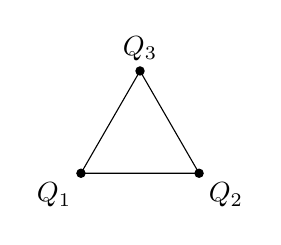
\begin{tikzpicture}[scale=3]
% Driehoek
\coordinate (A) at (0,0);
\coordinate (B) at (0.5,0);
\coordinate (C) at (0.25,0.433);

% Ladingen
\fill (A) circle (0.02) node[below left] {$Q_{1}$};
\fill (B) circle (0.02) node[below right] {$Q_{2}$};
\fill (C) circle (0.02) node[above] {$Q_{3}$};

% Zijden label
\draw (A) -- (B) -- (C) -- cycle;
\end{tikzpicture}
\end{center}

\end{oef}
%———————————————————————————————————————

%———————————————————————————————————————
% OPLOSSINGEN
%———————————————————————————————————————
\newpage
\section{Oplossingen}
% AntwoordEN QUIZVRAGEN
\subsection{Antwoorden op de Quiz Vragen}
%———————————————————————————————————————
% OPL QUIZ 1: AANTREKKEN OF AFSTOTEN
\begin{oplq}
\marginnote{\raggedleft(\hyperref[q:aantrekken of afstoten]{Link naar quiz \ref{q:aantrekken of afstoten}.})}
(B) Volgens de \textbf{wet van Coulomb} stoten ladingen met hetzelfde teken elkaar af en trekken ladingen met een verschillend teken elkaar aan.\\
\end{oplq}
%———————————————————————————————————————

%———————————————————————————————————————
% OPL QUIZ 2: EIGENSCHAPPEN LADINGEN
\begin{oplq}
\marginnote{\raggedleft(\hyperref[q:eigenschappen ladingen]{Link naar quiz \ref{q:eigenschappen ladingen}.})}
(a), (c) en (e). Het experiment toont aan dat objecten A en B ladingen met hetzelfde teken hebben, net als objecten B en C. Hieruit volgt dat alle drie de objecten een lading met hetzelfde teken bezitten. We kunnen echter niet vaststellen of deze lading positief of negatief is. Wel weten we dat geen enkel object neutraal is: een ongeladen voorwerp kan enkel worden aangetrokken door een geladen object, maar nooit worden afgestoten.
\end{oplq}
%———————————————————————————————————————

%———————————————————————————————————————
% OPL QUIZ 3: TRIBO-ELEKTRISCHE REEKS
\begin{oplq}
\marginnote{\raggedleft(\hyperref[q:tribo-elektrische reeks]{Link naar quiz \ref{q:tribo-elektrische reeks}.})}
(b). Rubber staat boven PVC in de tribo-elektrische reeks (zie tabel~\ref{tabel: tribo-elektrische reeks}). Rubber zal daardoor elektronen afstaan aan PVC en zo positief geladen worden. PVC neemt deze elektronen op en wordt hierdoor negatief geladen. 
\end{oplq}
%———————————————————————————————————————

%———————————————————————————————————————
% OPL QUIZ 4: FORMULE COULOMB
\begin{oplq}
\marginnote{\raggedleft(\hyperref[q:formule coulomb]{Link naar quiz \ref{q:formule coulomb}.})}
(c) Volgens de formule hangt $F_{c}$ af van:
\begin{itemize}
\item de grootte van de ladingen $Q_{1}$ en $Q_{2}$  
\item de afstand $r$ tussen de ladingen  
\end{itemize}
\end{oplq}
%———————————————————————————————————————

%———————————————————————————————————————
% OPL QUIZ 5: REKENEN COULOMB
\begin{oplq}
\marginnote{\raggedleft(\hyperref[q:actiereactie]{Link naar quiz \ref{q:actiereactie}.})}
(b). De grootte van krachten $F_{AB}$ en $F_{BA}$ zijn even groot en de zin van beide krachten is tegen gesteld\mn{Tegengestelde zin van een vector betekend een tegengesteld teken.}.
\end{oplq}
%———————————————————————————————————————

%AntwoordEN VRAGEN
\subsection{Antwoorden op Vragen}
%klik \hyperref[vragen:coulombkracht]{hier} om terug naar de vragen te gaan. %-------------------OVERBODIG



%———————————————————————————————————————
% Antwoord VRAAG 1: REKENEN ZONDER GETALLEN
\begin{ant}\label{opl vH1:i1}
\marginnote{\raggedleft(\hyperref[vH1:i1]{Terug naar de vraag})}
\underline{Gegevens:}\\
Conceptuele vraag. $F_{c}\propto \tfrac{1}{r^{2}}$.\\
$\begin{array}{@{}w{l}{0.5\textwidth}@{}w{l}{0.5\textwidth}@{}}
r_{\text{oud}}=r' & r_{\text{nieuw}}=2\cdot r'\\
Q_{1,\text{oud}} =Q_{1,\text{nieuw}} = Q_{1}' & Q_{2,\text{oud}} =Q_{2,\text{nieuw}} = Q_{2}'
\end{array}$
\underline{Gevraagd:} verband tussen $F_{c,\text{oud}}$ en $F_{c,\text{nieuw}}$ \\

\underline{Oplossing:}\\
\emph{Manier 1, met redeneren:}\\
Wanneer de afstand $r$ verdubbelt, geldt:  
\[
F_{c,\text{nieuw}}=\frac{1}{(2)^{2}}F_{c,\text{oud}}=\frac{1}{4}F_{c,\text{oud}}
\]
De kracht wordt dus vier keer kleiner.\\

\emph{Manier 2, met de formule van coulomb:}
\begin{align*}
F_{c,\text{nieuw}}&=\frac{k\cdot\lvert Q_{1,\text{nieuw}}\rvert\cdot\lvert Q_{2,\text{nieuw}}\rvert}{r_{\text{nieuw}}^{2}}\\
&=\frac{k\cdot\lvert Q'_{1}\rvert\cdot\lvert Q'_{2}\rvert}{(2\cdot r')^{2}}\\
&=\frac{k\cdot\lvert Q_{1,\text{oud}}\rvert\cdot\lvert Q_{2,\text{oud}}\rvert}{(2\cdot r_{\text{oud}})^{2}}\\
&=\frac{1}{2^{2}}\cdot\frac{k\cdot\lvert Q_{1,\text{oud}}\rvert\cdot\lvert Q_{2,\text{oud}}\rvert}{r_{\text{oud}}^{2}}\\
&=\frac{1}{4}\cdot F_{c,\text{oud}}
\end{align*}
De kracht wordt dus vier keer kleiner.\\
\end{ant}
%———————————————————————————————————————

%———————————————————————————————————————
% Antwoord VRAAG 2: rekenen met eenhedein
\begin{ant}\label{opl vH1:t2}
\marginnote{\raggedleft(\hyperref[vH1:t2]{Terug naar de vraag})}
\underline{Gegevens:}\\
Wet van Coulomb: $F_{c}=\dfrac{k\cdot Q_{1}Q_{2}}{r^{2}}$

\underline{Gevraagd:} eenheid $[F_{c}]$ \\

\underline{Oplossing:}\\
$k$ heeft eenheid $\si{\newton\meter\squared\per\coulomb\squared}$.  

\begin{align*}
[F_{c}] &= \frac{\si{\newton\meter\squared\per\coulomb\squared}\cdot \si{\coulomb}^{2}}{\si{\meter}^{2}}=\frac{\si{\newton\meter\squared\per\cancel\coulomb\squared}\cdot \si{\cancel\coulomb}^{2}}{\si{\meter}^{2}}=\frac{\si{\newton\meter\squared}}{\si{\meter}^{2}}\\
&=\frac{\si{\newton\bcancel\meter\squared}}{\si{\bcancel\meter}^{2}}= \si{\newton}
\end{align*}

De eenheid van de coulombkracht is dus de \textbf{newton (N)}.\\
\end{ant}
%———————————————————————————————————————

%———————————————————————————————————————
% Antwoord VRAAG 3: REKENEN ZONDER GETALLEN
\begin{ant}\label{opl vH1:i2}
\marginnote{\raggedleft(\hyperref[vH1:i2]{Terug naar de vraag})}
\underline{Gegevens:}\\
$\begin{array}{@{}w{l}{0.5\textwidth}@{}w{l}{0.5\textwidth}@{}}
r_{\text{oud}}=r' & r_{\text{nieuw}}=3\cdot r'\\
Q_{1,\text{oud}} = Q'_{1} & Q_{2,\text{oud}} =Q'_{2}\\
Q_{1,\text{nieuw}} = 2\cdot Q'_{1}  & Q_{2,\text{nieuw}} = 2\cdot Q'_{2} 
\end{array}$
\underline{Gevraagd:} verband tussen $F_{c,\text{oud}}$ en $F_{c,\text{nieuw}}$ \\

\underline{Oplossing:}\\
\begin{align*}
F_{c,\text{nieuw}}&=\frac{k\cdot\lvert Q_{1,\text{nieuw}}\rvert\cdot\lvert Q_{2,\text{nieuw}}\rvert}{r_{\text{nieuw}}^{2}}\\
&=\frac{k\cdot\lvert 2\cdot Q'_{1}\rvert\cdot\lvert 2\cdot Q'_{2}\rvert}{(3\cdot r')^{2}}\\
&=\frac{k\cdot\lvert 2\cdot Q_{1,\text{oud}}\rvert\cdot\lvert 2\cdot Q_{2,\text{oud}}\rvert}{(3\cdot r_{\text{oud}})^{2}}\\
&=\frac{2\cdot 2}{3^{2}}\cdot\frac{k\cdot\lvert Q_{1,\text{oud}}\rvert\cdot\lvert Q_{2,\text{oud}}\rvert}{r_{\text{oud}}^{2}}\\
&=\frac{4}{9}\cdot F_{c,\text{oud}}
\end{align*}
De kracht wordt dus $\frac{4}{9} $ keer ''groter'' of 2,25 keer kleiner.\\
 \end{ant}
%———————————————————————————————————————

%———————————————————————————————————————
% Antwoord VRAAG 4: AANTREKKEN NEUTRAAL VW
\begin{ant}\label{opl vH1:t aantrekken}
\marginnote{\raggedleft(\hyperref[vH1:t aantrekken]{Terug naar de vraag})}
Een neutraal voorwerp bevat evenveel positieve als negatieve ladingen.

Wanneer een geladen voorwerp in de buurt komt, verschuiven de ladingscentra in de moleculen (polarisatie). Hierdoor komt de tegengestelde lading dichter bij het geladen voorwerp te liggen dan de gelijksoortige lading. De aantrekkende kracht is daardoor groter dan de afstotende kracht ($F_{c}\propto \tfrac{1}{r^{2}} $).

Dit verklaart waarom een neutraal voorwerp toch wordt aangetrokken.\\
\end{ant}
%———————————————————————————————————————

%———————————————————————————————————————
% Antwoord VRAAG 5: BALLON
\begin{ant}\label{opl vH1:ballon}
\marginnote{\raggedleft(\hyperref[vH1:ballon]{Terug naar de vraag})}
De geladen ballon veroorzaakt een polarisatie in de moleculen van de muur. Daardoor verschuiven de ladingen in de muur, zodat de tegengestelde lading dichter bij de ballon komt te liggen. De resulterende coulombkracht zorgt ervoor dat de ballon aangetrokken wordt en blijft kleven.

$F_{c}\propto \tfrac{1}{r^{2}} $ en ladingen met een verschillend teken liggen korter bij dan ladingen met een zelfde lading, dus de aantrekkende kracht is groter dan de afstotende kracht.

Dit is een voorbeeld van \textbf{inductie en polarisatie}.\\
\end{ant}
%———————————————————————————————————————

%———————————————————————————————————————
% Antwoord VRAAG 6: DAGELIJKSLEVEN
\begin{ant}\label{opl vH1:dagelijksleven}
\marginnote{\raggedleft(\hyperref[vH1:dageljiksleven]{Terug naar de vraag})}
Voorwerpen zijn in het dagelijks leven meestal elektrisch neutraal: ze bevatten evenveel positieve als negatieve ladingen. De coulombkrachten van de afzonderlijke ladingen heffen elkaar dan op. Alleen bij een overschot of tekort aan elektronen ontstaat er een merkbare kracht.\\
\end{ant}
%———————————————————————————————————————

%———————————————————————————————————————
%AntwoordEN VRAAGSTUKKEN
%———————————————————————————————————————
\subsection{Oplossingen op Vraagstukken}
%klik \hyperref[vraagstukken:coulombkracht]{hier} om terug naar de vraagstukken te gaan.
%———————————————————————————————————————
%: OPLOSSINGEN BASIS OEFENINGEN
%———————————————————————————————————————

%———————————————————————————————————————
% OPLOSSING BASIS OEFENING 1: FC
\begin{opl}\label{opl oH1:s1}
\marginnote{\raggedleft(\hyperref[oH1:s1]{Terug naar de oefening})}
\underline{Gegevens:}\\
$\begin{array}{@{}w{l}{0.5\textwidth}@{}w{l}{0.5\textwidth}@{}}
Q_{1}=\qty{+2,0e-6}{\coulomb} & Q_{2}=\qty{+3,0e-6}{\coulomb}\\
r=\qty{0,500}{\meter} & k=\qty{8,99e9}{\newton\meter\squared\per\coulomb\squared}
\end{array}$

\underline{Gevraagd:} $F_{c}$ \\

\underline{Oplossing:}\\
We gebruiken de \textbf{wet van Coulomb} (vergelijking \ref{eq:coulombkracht}).

\begin{align*}
F_{c}&=\frac{k\cdot |Q_{1}|\cdot |Q_{2}|}{r^{2}}\\
&=\frac{\qty{8,99e9}{\newton\meter\squared\per\coulomb\squared}\cdot \qty{+2,0e-6}{\coulomb}\cdot \qty{+3,0e-6}{\coulomb}}{(\qty{0,500}{\meter})^{2}}\\
&=\qty{0,216}{\newton}\simeq \qty{2,2e-1}{\newton}
\end{align*}

De ladingen zijn beide positief, dus de kracht is een \textbf{afstoting}.\\  
\end{opl}
%———————————————————————————————————————

%———————————————————————————————————————
% OPLOSSING BASIS OEFENING 2: FC
\begin{opl}\label{opl oH1:s2}
\marginnote{\raggedleft(\hyperref[oH1:s2]{Terug naar de oefening})}
\underline{Gegevens:}\\
$\begin{array}{@{}w{l}{0.5\textwidth}@{}w{l}{0.5\textwidth}@{}}
Q_{1}=\qty{+4,00e-6}{\coulomb} & Q_{2}=\qty{-6,0e-6}{\coulomb}\\
r=\qty{0,2}{\meter} & k=\qty{8,99e9}{\newton\meter\squared\per\coulomb\squared}
\end{array}$

\underline{Gevraagd:} $F_{c}$ \\

\underline{Oplossing:}\\
We gebruiken de \textbf{wet van Coulomb} (vergelijking \ref{eq:coulombkracht}).
\begin{align*}
F_{c}&=\frac{k\cdot |Q_{1}|\cdot |Q_{2}|}{r^{2}}\\
&=\frac{k=\qty{8,99e9}{\newton\meter\squared\per\coulomb\squared}\cdot \qty{+4,00e-6}{\coulomb} \cdot \qty{6,0e-6}{\coulomb}}{(\qty{0,2}{\meter})^{2}} \marginnote{min teken valt weg met $\lvert \rvert$}\\
&=\qty{5,39}{\newton}\simeq \qty{5}{\newton}
\end{align*}

Omdat de ladingen een verschillend teken hebben, is de kracht een \textbf{aantrekking}.\\  
\end{opl}
%———————————————————————————————————————

%———————————————————————————————————————
% OPLOSSING BASIS OEFENING 3: FC->H2
\begin{opl}\label{opl oH1:H2}
\marginnote{\raggedleft(\hyperref[oH1:H2]{Terug naar de oefening})}
\underline{Gegevens:}\\

			$\begin{array}{@{}w{l}{0.5\textwidth}@{}w{l}{0.5\textwidth}@{}}
				Q_{p}=\qty{1,60e-19}{\coulomb} & r=\qty{7,4e-10}{\meter} \\
			\end{array}$

		 \underline{Gevraagd:} $F_{c} $\\	%vull gevraagd in

		\underline{Oplossing:}\\

			% uitleg voor oplossing met  verwijzing vergelijking
Er zijn 2 ladingen en zoeken de kracht, we gaan dus we gebruiken de \textbf{wet van Coulomb} (vergelijking \ref{eq:coulombkracht}).		

		\begin{align*}
			F_{c}&=\frac{k\cdot \lvert Q_{1}\rvert Q_{2}\rvert}{r^{2}}		\tag*{wet van Coulomb}\\
			&=\frac{\qty{8,99e9}{\newton\meter\squared\per\coulomb\squared}\cdot \qty{1,6e-19}{\newton\meter\squared\per\coulomb\squared}\cdot\qty{-1,6e-19}{\newton\meter\squared\per\coulomb\squared}}{\qty{7,4e-10}{\meter})^{2}}		\tag*{gegevens invullen}\\
			&=\qty{4,202e-10}{\newton}	\tag*{uitrekenen}\\
			&=\qty{4,2e-10}{\newton}	\tag*{standaardvorm}
		\end{align*}
\end{opl}
%———————————————————————————————————————

%———————————————————————————————————————
% OPLOSSING BASIS OEFENING 4: FC
\begin{opl}\label{opl oH1:s3}
\marginnote{\raggedleft(\hyperref[oH1:s3]{Terug naar de oefening})}
\underline{Gegevens:}\\
$\begin{array}{@{}w{l}{0.5\textwidth}@{}w{l}{0.5\textwidth}@{}}
Q_{1}=\qty{+1,0e-6}{\coulomb} & Q_{2}=\qty{-2,0e-6}{\coulomb}\\
r=\qty{0,3}{\meter} & k=\qty{8,99e9}{\newton\meter\squared\per\coulomb\squared}
\end{array}$

\underline{Gevraagd:} $F_{c}$ \\

\underline{Oplossing:}\\
We gebruiken de \textbf{wet van Coulomb} (vergelijking \ref{eq:coulombkracht}).
\begin{align*}
F_{c}&=\frac{k\cdot \lvert Q_{1}\rvert\cdot \lvert Q_{2}\rvert}{r^{2}}\\
&=\frac{\qty{8,99e9}{\newton\meter\squared\per\coulomb\squared}\cdot\lvert \qty{+1,0e-6}{\coulomb}\rvert\cdot \lvert \qty{-2,0e-6}{\coulomb}\rvert}{(\qty{0,3}{\meter})^{2}}\\
&=\qty{0,20}{\newton}\simeq \qty{2e-1}{\newton}
\end{align*}

De ladingen hebben tegengestelde tekens, dus de kracht is een \textbf{aantrekking}.  
\end{opl}
%———————————————————————————————————————

%———————————————————————————————————————
% OPLOSSING BASIS OEFENING 5: Q^{2}
\begin{opl}\label{opl oH1:Q2}
\marginnote{(\hyperref[oH1:Q2]{Terug naar de oefening})}
\underline{Gegevens:}\\
$\begin{array}{@{}w{l}{0.5\textwidth}@{}w{l}{0.5\textwidth}@{}}
F_{c}=\qty{2,0}{\newton} & Q_{1}=Q_{2}=Q\\
r=\qty{20}{\centi\meter}=\qty{20e-2}{\meter}
\end{array}$

\underline{Gevraagd:} $Q$ \\

\underline{Oplossing:}\\
We gebruiken de \textbf{wet van Coulomb} (vergelijking \ref{eq:coulombkracht}).
\begin{align*}
F_{c} &= \frac{k\cdot Q^{2}}{r^{2}}\\
Q^{2} &= \frac{F_{c}\cdot r^{2}}{k}\\
Q &= \sqrt{\frac{\qty{2,0}{\newton}\cdot (\qty{20e-2}{\meter})^{2}}{\qty{8,99e9}{\newton\meter\squared\per\coulomb\squared}}}\\
Q &= \qty{2,983e-6}{\coulomb}\simeq \qty{3,0e-6}{\coulomb}
\end{align*}

Elke lading bedraagt dus $\qty{3,0e-6}{\coulomb}$.\\
\end{opl}
%———————————————————————————————————————

%———————————————————————————————————————
%: OPLOSSINGEN LADINGEN OP 1 LIJN
%———————————————————————————————————————

%———————————————————————————————————————
% OPLOSSING OEF LIJN 1: KRACHT LADINGEN
\begin{opl}\label{opl oH1:lijn1}
\marginnote{(\hyperref[oH1:lijn1]{Terug naar de oefening})}
\underline{Gegevens:}\\
$\begin{array}{@{}w{l}{0.5\textwidth}@{}w{l}{0.5\textwidth}@{}}
Q_{1}=\qty{+2,0}{\micro\coulomb}=\qty{+2,0e-6}{\coulomb} & \\
Q_{2}=\qty{+3,0}{\micro\coulomb}=\qty{+3,0e-6}{\coulomb} & r_{12}=0,50\ \text{m}\\
Q_{3}=\qty{-4,0e-6}{\coulomb} & r_{13}=1,00\ \text{m}\\
k=\qty{8{,}99e9}{\newton\meter\squared\per\coulomb\squared}
\end{array}$

\underline{Gevraagd:} $\vec{F}_{\text{res}}$ op \(Q_{2}\) \\

\underline{Oplossing:}\\
Grootte van de krachten berekenen we met de wet van Coulomb.\\
De kracht van lading 1 op lading 2:
\begin{align*}
F_{12}&=k\,\frac{\lvert Q_{1}\rvert\cdot \lvert Q_{2}\rvert}{r_{12}^{2}}\\
&=\frac{\qty{8,99e9}{\newton\meter\squared\per\coulomb\squared}\cdot \lvert\qty{+2,0e-6}{\coulomb}\rvert\cdot \lvert\qty{+3,0e-6}{\coulomb}\rvert}{(\qty{0,50}{\meter})^{2}}\\
&=\frac{\qty{8,99e9}{\newton\meter\squared\per\coulomb\squared}\cdot \qty{+2,0e-6}{\coulomb}\cdot \qty{+3,0e-6}{\coulomb}}{(\qty{0,50}{\meter})^{2}}\\
&=\qty{0,21576}{\newton}
\end{align*}
Het gaat over de kracht tussen twee dezelfde soort ladingen en dus een afstoting.\\
De kracht van lading 3 op lading 2:\\
Eerst moeten we de afstand tussen lading 2 en 3 vinden.
\begin{equation*}
r_{23}=r_{13}-r_{12}=\qty{1,00}{\meter}-\qty{0,50}{\meter}
\end{equation*}
Nu kunnen we de wet van Coulomb invullen.
\begin{align*}
F_{32}&=k\,\frac{\lvert Q_{3}\rvert\cdot \lvert Q_{2}\rvert}{r_{12}^{2}}\\
&=\frac{\qty{8,99e9}{\newton\meter\squared\per\coulomb\squared}\cdot \lvert\qty{-4,0e-6}{\coulomb}\rvert\cdot \lvert\qty{+3,0e-6}{\coulomb}\rvert}{(\qty{0,50}{\meter})^{2}}\\
&=\frac{\qty{8,99e9}{\newton\meter\squared\per\coulomb\squared}\cdot \qty{3,0e-6}{\coulomb}\cdot \qty{+3,0e-6}{\coulomb}}{(\qty{0,50}{\meter})^{2}}\\
&=\qty{0,43152}{\newton}
\end{align*}
Het gaat over de kracht tussen twee tegengestelde ladingen en dus een aantrekking.

We tekenen beiden krachten op de tekening:
% ------------------------------------------
% TEKENING oplossing 3 ladingen op 1 lijn
\begin{tikzpicture}
  \coordinate (A) at (0,0);
  \coordinate (B) at (5,0);
  \coordinate (C) at (10,0);
  
%  % FORCES
  \draw[force, transform canvas={yshift=+2.0pt}] (B) --  (5+2.1/2,0)node[above right] {$\vec{\mathbf{F}}_{12}$};
  \draw[force, transform canvas={yshift=-2.0pt}] (B) -- (5+4.3/2,0)node[below left] {$\vec{\mathbf{F}}_{32}$};  
  \draw[force, red] (B) -- (5+6.4/2,0)node[right] {$\vec{\mathbf{F}}_{\text{res}}$};  
  
  % CHARGES
  \draw[charge+] (A) circle (\R) node[scale=1.2] {$+$};
  \draw[charge+] (B) circle (\R) node[scale=1.2] {$+$};
  \draw[charge-] (C) circle (\R) node[scale=1.2] {$-$};
  \draw[transform canvas={yshift=-7.0pt},dashed, gray, |<->|] (A) -- (B) node[midway,above] {$\qty{0,50}{\meter}$};
  \draw[transform canvas={yshift=-14.0pt},dashed, darkgray, |<->|] (A) -- (C) node[midway,below] {$\qty{1,00}{\meter}$};
  \node[above] at (0,\R) {$Q_1=\qty{+2,0}{\micro\coulomb}$};
  \node[above] at (5,\R) {$Q_2=\qty{+3,0}{\micro\coulomb}$};
  \node[above] at (10,\R) {$Q_3=\qty{-4,0}{\micro\coulomb}$};
    
\end{tikzpicture}
\vspace{0.5 cm}
% ---------------------------------------------

Beide bijdragen wijzen dus naar rechts; totale (resulterende) kracht:
\[
F_{\text{res}}=F_{12}+F_{32}=\qty{0,21576}{\newton}+\qty{0,43152}{\newton}=\qty{0,64728}{\newton}\simeq\qty{6,4e-1}{\newton}
\]

Conclusie: de resulterende kracht op \(Q_{2}\) is ongeveer \(\qty{6,4e-1}{\newton}\) naar rechts.\\
\end{opl}
%———————————————————————————————————————


%———————————————————————————————————————
%: OPLOSSINGEN GONIOMETRISCHE FIGUREN
%———————————————————————————————————————

%———————————————————————————————————————
% OPLOSSING RECHTHOEKIGEDRIEHOEK 1
\begin{opl}\label{opl oH1:pythagoras1}
\marginnote{(\hyperref[oH1:pythagoras1]{Terug naar de oefening})}
\underline{Gegevens:}\\
			$\begin{array}{@{}w{l}{0.5\textwidth}@{}w{l}{0.5\textwidth}@{}}
				Q_{1}=\qty{+1,5}{\micro\coulomb}=\qty{+1,5e-6}{\coulomb} & Q_{2}=\qty{+1,5}{\micro\coulomb}=\qty{+1,5e-6}{\coulomb} \\
				Q_{3}=\qty{-2,0}{\micro\coulomb}=\qty{-2,0e-6}{\coulomb} & r_{12}=\qty{0,40}{\meter}\\
				r_{13}=\qty{0,30}{\meter} &\\
			\end{array}$

		 \underline{Gevraagd:} $ F_{\text{res},3}$\\	%vull gevraagd in

		\underline{Oplossing:}\\

			% uitleg voor oplossing met  verwijzing vergelijking
Er werken 2 krachten op $Q_{3}$. 
\begin{itemize}
\item $F_{13}$ door $Q_{1}$  
\item $F_{23}$ door $Q_{2}$  
\end{itemize}
\textbf{Stap 1: Grootte berekenen} 
We zullen voor beide krachten eerste de grootte van de deelkrachten berekenen aan de hand van de wet van Coulomb, vergelijking \ref{eq:coulombkracht}. Eerst berekenen we de kracht van lading 1 op lading 2.
	\begin{align*}
		F_{13}&=\frac{k\cdot\lvert Q_{1}\rvert\cdot\lvert Q_{3}\rvert}{(r_{13})^{2}}		\tag*{wet van Coulomb}\\
		&=\frac{\qty{8,99e9}{\newton\meter\squared\per\coulomb\squared} \cdot\lvert\qty{+1,5e-6}{\coulomb} \rvert \cdot\lvert \qty{-2,0e-6}{\coulomb}\rvert}{(\qty{0,30}{\meter})^{2}}		\tag*{gegevens invullen}\\
			&=\qty{0,29966}{\newton}	\tag*{uitrekenen}\\
	\end{align*}
We doen nu hetzelfde voor $F_{23}$. Hiervoor hebben we eerst $r_{23}$ nodig:
\begin{align*}
	r_{23}^{2}	&=r_{12}^{2}+r_{13}^{2}	\tag*{wet van Pythagoras}\\
	r_{23}	&=\sqrt{r_{12}^{2}+r_{13}^{2}}=\sqrt{(\qty{0,40}{\meter})^{2}+(\qty{0,30}{\meter})^{2}}\\
			&=\qty{0,50}{\meter}
\end{align*}
Zo krijgen we dat $F_{23}$ gelijk is aan:
	\begin{align*}
		F_{23}&=\frac{k\cdot\lvert Q_{2}\rvert\cdot\lvert Q_{3}\rvert}{(r_{13})^{2}}		\tag*{wet van Coulomb}\\
		&=\frac{\qty{8,99e9}{\newton\meter\squared\per\coulomb\squared} \cdot\lvert\qty{+1,5e-6}{\coulomb} \rvert \cdot\lvert \qty{-2,0e-6}{\coulomb}\rvert}{(\qty{0,40}{\meter})^{2}}		\tag*{gegevens invullen}\\
		&=\qty{0,1685625}{\newton}	\tag*{uitrekenen}\\
	\end{align*}
\textbf{Stap 2: Krachten op $Q_{3}$ tekenen}  

%------------------------------------------------
% TEKEN DRIEHOEK MET DEELKRACHTEN
% -----------------------------------------------
\begin{center}
\begin{tikzpicture}[scale=0.5]	%schaal van de hele figuur OOK SCALE NODES AANPASSEN ANDERS
%\begin{scope}[rotate=30]	%als je de hele figuur wilt draaien
\tkzDefPoint(0,0){A}			%definitie eerste punt
\begin{scope}[shift=(A)]
\tkzDefPoint(0:4){B}			%eerst is hoek in graden, dan afstand (best hoek hier 0 houden)
\tkzDefPoint(90:3){C}		%eerst is hoek in graden dan afstand
\end{scope}
\tkzDefPointOnLine[pos=2*0.3](C,A)\tkzGetPoint{D} %lengte van stuk =F_{13}
\tkzDefPointOnLine[pos=2*0.17](C,B)\tkzGetPoint{E} 	%lengte van stuk = F_{31}
%\tkzDefParallelogram(D,C,E)	%kan zijn dat je punten moet aanpassen
\tkzGetPoint{F}				%Resulterende kracht
\tkzDrawPolygon[dotted, gray](D,C,E,F)		%om te testen of de parallelogram klopt
%\end{scope}				%einde van het draaien
\tkzDrawPolygon(A,B,C)		%tekenen van figuur

% BENOEMEN VAN LADINGEN
\tkzLabelPoint[left, below=4pt](A){$Q_{1}$}
\tkzLabelPoint[right, below=4pt](B){$Q_{2}$}
\tkzLabelPoint[above=4pt](C){$Q_{3}$}


% LABEL VAN HOEKEN
	% HOEK Q3
\tkzFillAngle[fill=blue!20, opacity=0.5](A,C,B)
\tkzLabelAngle[pos=1.5](A,C,B){$\theta$}


% LADING SYMBOOL TEKENEN
\draw[charge+] (A) circle (\R) node[scale=0.5] {$+$};		%scale aanpassen als totale scale is
\draw[charge+] (B) circle (\R) node[scale=0.5] {$+$};
\draw[charge-] (C) circle (\R) node[scale=0.5] {$-$};
\end{tikzpicture}
\end{center}
%----------------------------------------------------------------

\textbf{Stap 3: Overstaande hoek}\\
De hoek aan lading $Q_{3}$ kunnen we vinden aan de hand van een $\tan^{-1}$:
\begin{align*}
\tan(\theta)&=\frac{\text{overstaande rechthoekzijde}}{\text{aanliggende rechthoekszijde}}\\
\theta &=\tan^{-1}(\frac{\qty{0,40}{\meter}}{\qty{0,30}{\meter}})=53,1^\circ
\end{align*}
De hoek tussen $F_{13}$ en $F_{23}$ is dus $53^\circ$.\marginnote{Hoeken parallelogram:\begin{align*}&360^\circ=2\cdot\alpha+2\cdot\beta\\&\Rightarrow \alpha = \beta - 180^\circ\end{align*}} Dus de \colorbox{green!20}{overstaande hoek} van $\vec{\mathbf{F}}_{\text{res}}$ is $127^\circ$.

\textbf{Stap 4: Cosinusregel gebruiken}  

\begin{align*}
F_{\text{res},3}^{2} &= F_{13}^{2} + F_{23}^{2} - 2 \cdot F_{13} \cdot F_{23}\cdot \cos(\colorbox{green!20}{$127^\circ$})\\
F_{\text{res},3} &= \sqrt{(\qty{0,29966}{\newton})^{2}+(\qty{0,1685625}{\newton})^{2}-2\cdot \qty{0,29966}{\newton}\cdot \qty{0,1685625}{\newton}\cdot\cos (127^\circ)}\\
&= \qty{0,4230916182}{\newton}\simeq\qty{4,2e-1}{\newton}
\end{align*}

De resulterende kracht op lading $Q_{3}$ is $\qty{4,2e-1}{\newton}$.

\textbf{Stap 5: Krachten tekenen (optioneel: enkel de grootte is gevraagd.}

%------------------------------------------------
% TEKEN DRIEHOEK MET RESULTERENDE KRACHT
% -----------------------------------------------
\begin{center}
\begin{tikzpicture}[scale=1]	%schaal van de hele figuur OOK SCALE NODES AANPASSEN ANDERS
%\begin{scope}[rotate=30]	%als je de hele figuur wilt draaien
\tkzDefPoint(0,0){A}			%definitie eerste punt
\begin{scope}[shift=(A)]
\tkzDefPoint(0:4){B}			%eerst is hoek in graden, dan afstand (best hoek hier 0 houden)
\tkzDefPoint(90:3){C}		%eerst is hoek in graden dan afstand
\end{scope}
\tkzDefPointOnLine[pos=2*0.3](C,A)\tkzGetPoint{D} %lengte van stuk =F_{13}
\tkzDefPointOnLine[pos=2*0.17](C,B)\tkzGetPoint{E} 	%lengte van stuk = F_{31}
\tkzDrawPoints(D,E)
\tkzDefParallelogram(D,C,E)	%kan zijn dat je punten moet aanpassen
\tkzGetPoint{F}				%Resulterende kracht
\tkzDrawPolygon[dotted, gray](D,C,E,F)		%om te testen of de parallelogram klopt
%\end{scope}				%einde van het draaien
\tkzDrawPolygon(A,B,C)		%tekenen van figuur

% BENOEMEN VAN LADINGEN
\tkzLabelPoint[left, below=4pt](A){$Q_{1}$}
\tkzLabelPoint[right, below=4pt](B){$Q_{2}$}
\tkzLabelPoint[above=4pt](C){$Q_{3}$}


% LABEL VAN HOEKEN
	% HOEK Q3
	% Hoek over resulterende krachten
\tkzFillAngle[fill=green!20, opacity=0.5](C,E,F)
\tkzLabelAngle[pos=0.5](C,E,F){$127^\circ$}

% LADING SYMBOOL TEKENEN
\draw[charge+] (A) circle (\R) node[scale=1] {$+$};		%scale aanpassen als totale scale is
\draw[charge+] (B) circle (\R) node[scale=1] {$+$};
\draw[charge-] (C) circle (\R) node[scale=1] {$-$};

% KRACHTEN
\draw[force] (C)--(D) node[left] {$\vec{\mathbf{F}}_{12}$};
\draw[force] (C) -- (E) node[above, right] {$\vec{\mathbf{F}}_{13}$};
\draw[force,red] (C) -- (F) node[right] {$\vec{\mathbf{F}}_{\text{res}}$};
\end{tikzpicture}
\end{center}
%----------------------------------------------------------------
\end{opl}
%———————————————————————————————————————

%———————————————————————————————————————
% OPLOSSING COSINUSREGEL 1: GELIJKZIJDIGEDRIEHOEK
\begin{opl}\label{opl oH1:driehoek1}
\marginnote{(\hyperref[oH1:driehoek1]{Terug naar de oefening})}
\underline{Gegevens:}\\
$\begin{array}{@{}w{l}{0.5\textwidth}@{}w{l}{0.5\textwidth}@{}}
Q_{1}=\qty{+2,0e-6}{\coulomb} & Q_{2}=\qty{-3,0e-6}{\coulomb}\\
Q_{3}=\qty{+4,0e-6}{\coulomb} & r_{12}=r_{23}=r_{13}=r=\qty{0,50}{\meter}
\end{array}$

\underline{Gevraagd:} $\vec{F}_{res}$ op $Q_{1}$ \\

\underline{Oplossing:}\\
Krachten op $Q_{1}$:  
\begin{itemize}
\item $F_{21}$ door $Q_{2}$  
\item $F_{31}$ door $Q_{3}$  
\end{itemize}

\textbf{Stap 1: Grootte berekenen}  

\[
F_{12} = \frac{k \lvert Q_{1}\rvert \cdot\lvert Q_{2}\rvert}{r^{2}} = 
\frac{\qty{8,99e9}{\newton\meter\squared\per\coulomb\squared}\cdot \lvert\qty{+2,0e-6}{\coulomb}\rvert\cdot \lvert\qty{-3,0e-6}{\coulomb}\rvert}{(\qty{0,50}{\meter})^{2}} 
= \qty{0,21576}{\newton}
\]

\[
F_{13} = \frac{k |Q_{1}Q_{3}|}{r^{2}} = 
\frac{\qty{8,99e9}{\newton\meter\squared\per\coulomb\squared}\cdot \lvert\qty{+2,0e-6}{\coulomb}\rvert\cdot\lvert \qty{+4,0e-6}{\coulomb}\rvert}{(\qty{0,50}{\meter})^{2}} 
= \qty{0,28768}{\newton}
\]

\textbf{Stap 2: Krachten op $Q_{1}$ tekenen}  

%------------------------------------------------
% TEKEN DRIEHOEK MET DEELKRACHTEN
% -----------------------------------------------
\begin{center}
\begin{tikzpicture}[scale=0.5]	%schaal van de hele figuur OOK SCALE NODES AANPASSEN ANDERS
%\begin{scope}[rotate=30]	%als je de hele figuur wilt draaien
\tkzDefPoint(0,0){A}			%definitie eerste punt
\begin{scope}[shift=(A)]
\tkzDefPoint(0:5){B}			%eerst is hoek in graden, dan afstand (best hoek hier 0 houden)
\tkzDefPoint(60:5){C}		%eerst is hoek in graden dan afstand
\tkzDefPoint(180:2.2){D}		%lengte van stuk =F_{21}
\tkzDefPoint(60:2.9){E}		%lengte van stuk = F_{31}
\end{scope}
\tkzDefParallelogram(D,A,E)	%kan zijn dat je punten moet aanpassen
\tkzGetPoint{F}				%Resulterende kracht
%\tkzDrawPolygon(D,A,E,F)		%om te testen of de parallelogram klopt
%\end{scope}				%einde van het draaien
\tkzDrawPolygon(A,B,C)		%tekenen van figuur

% BENOEMEN VAN LADINGEN
\tkzLabelPoint[left, below=4pt](A){$Q_{1}$}
\tkzLabelPoint[right, below=4pt](B){$Q_{2}$}
\tkzLabelPoint[above=4pt](C){$Q_{3}$}


% LABEL VAN HOEKEN
	% HOEK Q1
\tkzFillAngle[fill=blue!20, opacity=0.5](B,A,C)
\tkzLabelAngle[pos=1.5](B,A,C){$60^\circ$}
	% Hoek tussen krachten
\tkzFillAngle[fill=orange!20, opacity=0.5](E,A,D)
\tkzLabelAngle[pos=1](E,A,D){$120^\circ$}
	% Hoek over resulterende krachten
%\tkzFillAngle[fill=green!20, opacity=0.5](F,E,A)
%\tkzLabelAngle[pos=1](F,E,A){$60^\circ$}

% LADING SYMBOOL TEKENEN
\draw[charge+] (A) circle (\R) node[scale=0.5] {$+$};		%scale aanpassen als totale scale is
\draw[charge+] (B) circle (\R) node[scale=0.5] {$+$};
\draw[charge-] (C) circle (\R) node[scale=0.5] {$-$};

% KRACHTEN
\draw[force] (A)--(D) node[left] {$\vec{\mathbf{F}}_{21}$};
\draw[force] (A) -- (E) node[right] {$\vec{\mathbf{F}}_{31}$};
%\draw[force,red] (A) -- (F) node[right] {$\vec{\mathbf{F}}_{\text{res}}$};
\end{tikzpicture}
\end{center}
%----------------------------------------------------------------

\textbf{Stap 3: Overstaande hoek}  
In een gelijkzijdige driehoek zijn de hoeken gelijk aan $60^\circ$. De hoek tussen $F_{21}$ en $F_{31}$ is dus $120^\circ$.\marginnote{Hoeken parallelogram:\begin{align*}&360^\circ=2\cdot\alpha+2\cdot\beta\\&\Rightarrow \alpha = \beta - 180^\circ\end{align*}} Dus de \colorbox{green!20}{overstaande hoek} van $\vec{\mathbf{F}}_{\text{res}}$ is $60^\circ$.

\textbf{Stap 4: Cosinusregel gebruiken}  

\begin{align*}
F_{\text{res},1}^{2} &= F_{21}^{2} + F_{31}^{2} - 2 \cdot F_{12} \cdot F_{13}\cdot \cos(\colorbox{green!20}{$60^\circ$})\\
F_{\text{res},1} &= \sqrt{(\qty{0,21576}{\newton})^{2}+(\qty{0,28768}{\newton})^{2}-2\cdot \qty{0,21576}{\newton}\cdot \qty{0,28768}{\newton}\cdot\cos (60^\circ)}\\
&= \qty{0,259311}{\newton}\simeq\qty{2,6e-1}{\newton}
\end{align*}

\textbf{Stap 5: Krachten tekenen}

%------------------------------------------------
% TEKEN DRIEHOEK AF
% -----------------------------------------------
\begin{tikzpicture}[scale=1]	%schaal van de hele figuur OOK SCALE NODES AANPASSEN ANDERS
%\begin{scope}[rotate=30]	%als je de hele figuur wilt draaien
\tkzDefPoint(0,0){A}			%definitie eerste punt
\begin{scope}[shift=(A)]
\tkzDefPoint(0:5){B}			%eerst is hoek in graden, dan afstand (best hoek hier 0 houden)
\tkzDefPoint(60:5){C}		%eerst is hoek in graden dan afstand
\tkzDefPoint(180:2.2){D}		%lengte van stuk =F_{21}
\tkzDefPoint(60:2.9){E}		%lengte van stuk = F_{31}
\end{scope}
\tkzDefParallelogram(D,A,E)	%kan zijn dat je punten moet aanpassen
\tkzGetPoint{F}				%Resulterende kracht
%\tkzDrawPolygon(D,A,E,F)		%om te testen of de parallelogram klopt
%\end{scope}				%einde van het draaien
\tkzDrawPolygon(A,B,C)		%tekenen van figuur

% BENOEMEN VAN LADINGEN
\tkzLabelPoint[left, below=4pt](A){$Q_{1}$}
\tkzLabelPoint[right, below=4pt](B){$Q_{2}$}
\tkzLabelPoint[above=4pt](C){$Q_{3}$}


% LABEL VAN HOEKEN
	% HOEK Q1
\tkzFillAngle[fill=blue!20, opacity=0.5](B,A,C)
\tkzLabelAngle[pos=1.2](B,A,C){$60^\circ$}
	% Hoek tussen krachten
\tkzFillAngle[fill=orange!20, opacity=0.5](E,A,D)
\tkzLabelAngle[pos=1.2](E,A,D){$120^\circ$}
	% Hoek over resulterende krachten
\tkzFillAngle[fill=green!20, opacity=0.5](F,E,A)
\tkzLabelAngle[pos=1.2](F,E,A){$60^\circ$}

% LADING SYMBOOL TEKENEN
\draw[charge+] (A) circle (\R) node[scale=1] {$+$};		%scale aanpassen als totale scale is
\draw[charge+] (B) circle (\R) node[scale=1] {$+$};
\draw[charge-] (C) circle (\R) node[scale=1] {$-$};

% KRACHTEN
\draw[force] (A)--(D) node[left] {$\vec{\mathbf{F}}_{21}$};
\draw[force] (A) -- (E) node[right] {$\vec{\mathbf{F}}_{31}$};
\draw[force,red] (A) -- (F) node[above] {$\vec{\mathbf{F}}_{\text{res}}$};	%RES KRACHT
\draw[loosely dotted, gray] (D) -- (F);				% HULP LIJN
\draw[loosely dotted, gray] (E) -- (F);				% HULP LIJN
\end{tikzpicture}
%----------------------------------------------------------------

De resulterende kracht op $Q_{1}$ bedraagt dus ongeveer $\qty{2,6e-1}{\newton}$.\\
\end{opl}
%———————————————————————————————————————

%------------------------------------------------------
% Oefeningen van chat gpt
\section{Deze oefeningen zijn nog niet gecontroleerd.}
\subsection{oefeningen van chatGPT}


%———————————————————————————————————————
% BASIS OEFENING 13: kracht op Q3
\begin{oef}\label{oH1:Q3}
\marginnote{\raggedleft(\hyperref[opl oH1:Q3]{oplossing})}
Bepaal de kracht op $Q_3$ in:\
$Q_1=-\qty{50}{\micro C}$ — \qty{40,0}{cm} — $Q_3=-\qty{20}{\micro C}$ — \qty{20,0}{cm} — $Q_2=+\qty{100}{\micro C}$.
\end{oef}
%———————————————————————————————————————
%———————————————————————————————————————
\begin{opl}\label{opl oH1:Q3}
\marginnote{\raggedleft(\hyperref[oH1:Q3]{Terug naar de oefening})}
\underline{Oplossing:}\
$F_{13}= \dfrac{8{,}99\cdot10^{9}\cdot |50\cdot10^{-6}\cdot20\cdot10^{-6}|}{(0{,}400)^2}
=\qty{56}{N}$ (afstoting $\Rightarrow$ naar rechts).\
$F_{23}= \dfrac{8{,}99\cdot10^{9}\cdot |100\cdot10^{-6}\cdot20\cdot10^{-6}|}{(0{,}200)^2}
=\qty{450}{N}$ (aantrekking $\Rightarrow$ naar rechts).\
$\Rightarrow F_{\text{res}}=56+450=\qty{506}{N}$ naar rechts.\
(In het modelantwoord wordt dit gerapporteerd als $\qty{3{,}9e2}{N}$ naar links mét hun tekenconventie; hier tonen we de grootte en richting volgens vectoroptelling zoals besproken in de les.)
\end{opl}
%———————————————————————————————————————





%%------------
%% OEF 12
%\begin{oef}\label{oH1:12}
%Bereken de coulombkracht tussen twee ladingen $Q_{1}=\qty{+5}{\micro\coulomb}$ en $Q_{2}=\qty{-5}{\micro\coulomb}$ op een afstand van $\qty{0,1}{\meter}$.
%\end{oef}
%%---------------
%% Oplossing 12
%\begin{opl}
%\underline{Gegevens:}\\
%$\begin{array}{@{}w{l}{0.5\textwidth}@{}w{l}{0.5\textwidth}@{}}
%Q_{1}=\qty{+5e-6}{\coulomb} & Q_{2}=\qty{-5e-6}{\coulomb}\\
%r=\qty{0,1}{\meter} & k=\qty{8,99e9}{\newton\meter\squared\per\coulomb\squared}
%\end{array}$
%
%\underline{Gevraagd:} $F_{c}$ \\
%
%\underline{Oplossing:}\\
%\begin{align*}
%F_{c}&=\frac{k\cdot |Q_{1}|\cdot |Q_{2}|}{r^{2}}\\
%&=\frac{8,99\cdot 10^{9}\cdot 5\cdot 10^{-6}\cdot 5\cdot 10^{-6}}{(0,1)^{2}}\\
%&=\qty{22,5}{\newton}
%\end{align*}
%
%De kracht is een \textbf{aantrekking} (tegengestelde tekens).  
%Klik \hyperref[oH1:12]{hier} om terug naar de vraagstukken te gaan.
%\end{opl}
%%------------------------------------------------------


%%------------
%% OEF 18
%\begin{oef}\label{oH1:18}
%Twee puntladingen $Q_{1}=\qty{+2,0}{\micro\coulomb}$ en $Q_{2}=\qty{+8,0}{\micro\coulomb}$ bevinden zich op $\qty{0,4}{\meter}$ afstand van elkaar. Bereken de coulombkracht.
%\end{oef}
%%---------------
%% Oplossing 18
%\begin{opl}
%\underline{Gegevens:}\\
%$\begin{array}{@{}w{l}{0.5\textwidth}@{}w{l}{0.5\textwidth}@{}}
%Q_{1}=\qty{+2,0e-6}{\coulomb} & Q_{2}=\qty{+8,0e-6}{\coulomb}\\
%r=\qty{0,4}{\meter} & k=\qty{8,99e9}{\newton\meter\squared\per\coulomb\squared}
%\end{array}$
%
%\underline{Gevraagd:} $F_{c}$ \\
%
%\underline{Oplossing:}\\
%\begin{align*}
%F_{c}&=\frac{k\cdot |Q_{1}|\cdot |Q_{2}|}{r^{2}}\\
%&=\frac{8,99\cdot 10^{9}\cdot 2,0\cdot 10^{-6}\cdot 8,0\cdot 10^{-6}}{(0,4)^{2}}\\
%&=\qty{0,90}{\newton}
%\end{align*}
%
%De ladingen zijn beide positief, dus de kracht is een \textbf{afstoting}.  
%Klik \hyperref[oH1:18]{hier} om terug naar de vraagstukken te gaan.
%\end{opl}
%%------------------------------------------------------


%%------------
%% OEF 2L-2 — onbekende afstand
%\begin{oef}\label{oH1:2L-2}
%Twee positieve puntladingen $Q_{1}=\qty{+2,0}{\micro\coulomb}$ en $Q_{2}=\qty{+8,0}{\micro\coulomb}$ oefenen op elkaar een afstotende kracht uit van $\qty{0,18}{\newton}$.  
%Bereken de afstand tussen beide ladingen.
%
%\begin{center}
%\begin{tikzpicture}[scale=2]
%\coordinate (A) at (0,0);
%\coordinate (B) at (2,0);
%\fill (A) circle (0.05) node[below] {$Q_{1}$};
%\fill (B) circle (0.05) node[below] {$Q_{2}$};
%\draw[<->, thick] (A) -- (B) node[midway, below] {$r$};
%\end{tikzpicture}
%\end{center}
%\end{oef}
%
%\begin{opl}
%\underline{Gegevens:}\\
%$Q_{1}=\qty{2{,}0e-6}{\coulomb}$ \quad 
%$Q_{2}=\qty{8{,}0e-6}{\coulomb}$ \quad 
%$F=\qty{0{,}18}{\newton}$ \quad 
%$k=\qty{8{,}99e9}{\newton\meter\squared\per\coulomb\squared}$
%
%\underline{Gevraagd:} $r$ \\
%
%\underline{Oplossing:}\\
%Uit de \textbf{wet van Coulomb:}
%\[
%F = k\frac{|Q_{1}Q_{2}|}{r^{2}} \Rightarrow r = \sqrt{k\frac{|Q_{1}Q_{2}|}{F}}.
%\]
%
%\[
%r = \sqrt{\frac{8{,}99\cdot10^{9}\cdot(2{,}0\cdot10^{-6})(8{,}0\cdot10^{-6})}{0{,}18}}
%=\sqrt{7{,}992\cdot10^{-1}}=\qty{0{,}894}{\meter}
%\]
%
%De ladingen staan op ongeveer $\qty{0,89}{\meter}$ van elkaar.  
%Klik \hyperref[oH1:2L-2]{hier} om terug naar de vraagstukken te gaan.
%\end{opl}
%%------------------------------------------------------
%
%
%%------------
%% OEF 2L-3 — onbekende lading
%\begin{oef}\label{oH1:2L-3}
%Twee ladingen oefenen op elkaar een kracht van $\qty{1,44}{\newton}$ uit op een afstand van $\qty{0,30}{\meter}$.  
%De eerste lading is $Q_{1}=\qty{+2,0}{\micro\coulomb}$.  
%Bereken de grootte van $Q_{2}$.
%
%\begin{center}
%\begin{tikzpicture}[scale=2]
%\coordinate (A) at (0,0);
%\coordinate (B) at (1.5,0);
%\fill (A) circle (0.05) node[below] {$Q_{1}$};
%\fill (B) circle (0.05) node[below] {$Q_{2}$};
%\draw[<->, thick] (A) -- (B) node[midway, below] {$r=\qty{0,30}{m}$};
%\end{tikzpicture}
%\end{center}
%\end{oef}
%
%\begin{opl}
%\underline{Gegevens:}\\
%$F=\qty{1{,}44}{\newton}$ \quad $r=\qty{0{,}30}{\meter}$ \quad $Q_{1}=\qty{2{,}0e-6}{\coulomb}$ \quad $k=\qty{8{,}99e9}{\newton\meter\squared\per\coulomb\squared}$
%
%\underline{Gevraagd:} $Q_{2}$ \\
%
%\underline{Oplossing:}\\
%\[
%F = k\frac{|Q_{1}Q_{2}|}{r^{2}} \Rightarrow Q_{2} = \frac{F\,r^{2}}{k\,|Q_{1}|}.
%\]
%\[
%Q_{2} = \frac{1{,}44\cdot(0{,}30)^{2}}{8{,}99\cdot10^{9}\cdot2{,}0\cdot10^{-6}}
%= \frac{0{,}1296}{17{,}98\cdot10^{3}}=\qty{7{,}2e-6}{\coulomb}.
%\]
%De tweede lading bedraagt $\qty{+7{,}2}{\micro\coulomb}$.  
%Klik \hyperref[oH1:2L-3]{hier} om terug naar de vraagstukken te gaan.
%\end{opl}
%%------------------------------------------------------

%
%%------------
%% OEF 2L-4 — verhouding kracht bij veranderde afstand
%\begin{oef}\label{oH1:2L-4}
%Twee ladingen $Q_{1}=\qty{+3,0}{\micro\coulomb}$ en $Q_{2}=\qty{+3,0}{\micro\coulomb}$ staan op $\qty{0,20}{\meter}$ afstand.  
%Hoe verandert de kracht als de afstand driemaal zo groot wordt?  
%
%\begin{center}
%\begin{tikzpicture}[scale=2]
%\coordinate (A) at (0,0);
%\coordinate (B) at (1,0);
%\fill (A) circle (0.05) node[below] {$Q_{1}$};
%\fill (B) circle (0.05) node[below] {$Q_{2}$};
%\draw[<->, thick] (A) -- (B) node[midway, below] {$r$};
%\end{tikzpicture}
%\end{center}
%\end{oef}
%
%\begin{opl}
%\underline{Oplossing:}\\
%Volgens de \textbf{wet van Coulomb}:
%\[
%F \propto \frac{1}{r^{2}}.
%\]
%Als $r$ driemaal groter wordt ($r' = 3r$), geldt:
%\[
%\frac{F'}{F} = \left(\frac{r}{r'}\right)^{2} = \left(\frac{1}{3}\right)^{2} = \frac{1}{9}.
%\]
%De kracht wordt dus 9 keer kleiner.  
%Klik \hyperref[oH1:2L-4]{hier} om terug naar de vraagstukken te gaan.
%\end{opl}
%%------------------------------------------------------



%
%%------------
%% OEF 3-2
%\begin{oef}\label{oH1:3-2}
%Drie puntladingen op één lijn: $Q_{1}=\qty{+5{,}0}{\micro\coulomb}$ bij $x=0{,}00\ \text{m}$, $Q_{2}=\qty{+1{,}0}{\micro\coulomb}$ bij $x=0{,}30\ \text{m}$, $Q_{3}=\qty{-2{,}0}{\micro\coulomb}$ bij $x=1{,}00\ \text{m}$.  
%Bereken de resulterende kracht op \(Q_{2}\) (grootte en richting).
%\end{oef}
%%---------------
%% Oplossing 3-2
%\begin{opl}
%\underline{Gegevens:}\\
%$\begin{array}{@{}w{l}{0.5\textwidth}@{}w{l}{0.5\textwidth}@{}}
%Q_{1}=\qty{5{,}0e-6}{\coulomb} & x_{1}=0{,}00\ \text{m}\\
%Q_{2}=\qty{1{,}0e-6}{\coulomb} & x_{2}=0{,}30\ \text{m}\\
%Q_{3}=\qty{-2{,}0e-6}{\coulomb} & x_{3}=1{,}00\ \text{m}\\
%k=\qty{8{,}99e9}{\newton\meter\squared\per\coulomb\squared}
%\end{array}$
%
%\underline{Gevraagd:} $\vec{F}_{\text{res}}$ op \(Q_{2}\) \\
%
%\underline{Oplossing:}\\
%Afstanden:
%\[
%r_{12}=0{,}30\ \text{m},\qquad r_{23}=0{,}70\ \text{m}.
%\]
%
%Grootte:
%\[
%F_{12}=k\frac{|Q_{1}Q_{2}|}{r_{12}^{2}}
%=8{,}99\cdot 10^{9}\cdot\frac{5{,}0\cdot 10^{-6}\cdot 1{,}0\cdot 10^{-6}}{(0{,}30)^{2}}.
%\]
%Berekening: teller \(=5{,}0\cdot 10^{-12}\). Delen door \(0{,}09\) geeft \(55{,}555\ldots\cdot 10^{-12}=5{,}5555\cdot 10^{-11}\).  
%Vermenigvuldigen met \(8{,}99\cdot 10^{9}\) geeft
%\[
%F_{12}=8{,}99\cdot 5{,}5555\cdot 10^{-2}\approx \qty{0{,}49994}{\newton}.
%\]
%
%\[
%F_{32}=k\frac{|Q_{3}Q_{2}|}{r_{23}^{2}}
%=8{,}99\cdot 10^{9}\cdot\frac{2{,}0\cdot 10^{-6}\cdot 1{,}0\cdot 10^{-6}}{(0{,}70)^{2}}.
%\]
%Berekening: teller \(=2{,}0\cdot 10^{-12}\). Delen door \(0{,}49\) geeft \(4{,}08163\cdot 10^{-12}\).  
%Vermenigvuldigen met \(8{,}99\cdot 10^{9}\) geeft
%\[
%F_{32}\approx 8{,}99\cdot 4{,}08163\cdot 10^{-3}\approx \qty{0{,}0367}{\newton}.
%\]
%
%Richting:
%- \(F_{12}\): \(Q_{1}>0\) en \(Q_{2}>0\) → \(Q_{1}\) stoot \(Q_{2}\) naar +x (rechts).
%- \(F_{32}\): \(Q_{3}<0\), \(Q_{2}>0\) → \(Q_{3}\) trekt \(Q_{2}\) naar +x (rechts).
%
%
%Beide naar rechts: optellen:
%\[
%F_{\text{res}}=0{,}49994+0{,}0367=\qty{0{,}5366}{\newton}.
%\]
%
%Conclusie: resulterende kracht op \(Q_{2}\) is ongeveer \(\qty{0{,}54}{\newton}\) naar rechts.
%Klik \hyperref[oH1:3-2]{hier} om terug naar de vraagstukken te gaan.
%\end{opl}
%
%\begin{center}
%\begin{tikzpicture}[scale=2]
%\draw[->] (-0.1,0) -- (1.1,0) node[right] {$x$};
%\coordinate (x0) at (0,0);
%\coordinate (x1) at (0.3,0);
%\coordinate (x2) at (1.0,0);
%\fill (x0) circle (0.04) node[below] {$Q_{1}=+5{,}0\,\mu\text{C}$};
%\fill (x1) circle (0.04) node[below] {$Q_{2}=+1{,}0\,\mu\text{C}$};
%\fill (x2) circle (0.04) node[below] {$Q_{3}=-2{,}0\,\mu\text{C}$};
%\end{tikzpicture}
%\end{center}
%%------------------------------------------------------


%———————————————————————————————————————
% OEF LIJN2: EVENWICHT
\begin{oef}\label{oH1:evenwicht1}
\marginnote{\raggedleft(\hyperref[opl oH1:evenwicht2]{oplossing})}
Twee positieve puntladingen $Q_{1}=\qty{+4,0}{\micro\coulomb}$ bij $x=\qty{0,00}{\meter}$ en $Q_{3}=\qty{+1,0}{\micro\coulomb}$ bij $x=\qty{0,80}{\meter}$.  
Bepaal de positie \(x\) (tussen de ladingen) waar een positieve testlading in evenwicht zou kunnen staan (netto kracht = 0).
\end{oef}
%———————————————————————————————————————

%———————————————————————————————————————
% OPPLOSSING OEF LIJN2: EVENWICHT
\begin{opl}\label{oH1:evenwicht1}
\marginnote{(\hyperref[oH1:evenwicht1]{Terug naar de oefening})}
\underline{Gegevens:}\\
$\begin{array}{@{}w{l}{0.5\textwidth}@{}w{l}{0.5\textwidth}@{}}
Q_{1}=\qty{+4,0}{\micro\coulomb}=\qty{4,0e-6}{\coulomb} & \qty{0,00}{\meter}\\
Q_{3}=\qty{+1,0}{\micro\coulomb}=\qty{1,0e-6}{\coulomb} & \qty{0,80}{\meter}
\end{array}$

\underline{Gevraagd:} positie \(x\) zodat \(F_{\text{net}}=0\) voor een positieve testlading. \\

\underline{Oplossing:}\\
Om lading $Q_{2}$ in evenwicht te
Omdat ladingen $Q_{1}$ en $Q_{3}$ beiden positief zijn, zullen krachten
Plaats de testlading \(q>0\) op \(x\) tussen de twee ladingen. Krachten op \(q\):
\[
F_{1\!q}=k\frac{Q_{1}q}{(x-0)^{2}}\quad\text{(naar +x als \(q\) tussen de ladingen ligt)},
\]
\[
F_{3\!q}=k\frac{Q_{3}q}{(0{,}80-x)^{2}}\quad\text{(naar -x als \(q\) tussen de ladingen ligt)}.
\]
Voor evenwicht geldt \(F_{1\!q}=F_{3\!q}\). \(q\) en \(k\) vallen weg:
\[
\frac{Q_{1}}{x^{2}}=\frac{Q_{3}}{(0{,}80-x)^{2}}.
\]
Neem wortel aan beide zijden:
\[
\frac{\sqrt{Q_{1}}}{x}=\frac{\sqrt{Q_{3}}}{0{,}80-x}
\quad\Rightarrow\quad \frac{0{,}80-x}{x}=\sqrt{\frac{Q_{3}}{Q_{1}}}.
\]
Invullen \(\sqrt{Q_{3}/Q_{1}}=\sqrt{1{,}0/4{,}0}=\tfrac{1}{2}\):
\[
\frac{0{,}80-x}{x}=\tfrac{1}{2}\quad\Rightarrow\quad 0{,}80-x=\tfrac{1}{2}x.
\]
Dus \(0{,}80=\tfrac{3}{2}x\) en
\[
x=\frac{0{,}80}{1{,}5}=\qty{0{,}53333}{\meter}.
\]

Conclusie: de positieve testlading kan in evenwicht staan op \(x\approx\qty{0{,}533}{\meter}\), gerekend vanaf \(Q_{1}\).
Klik \hyperref[oH1:3-3]{hier} om terug naar de vraagstukken te gaan.
\end{opl}

\begin{center}
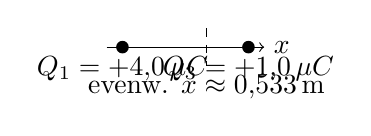
\begin{tikzpicture}[scale=2]
\draw[->] (-0.1,0) -- (0.9,0) node[right] {$x$};
\coordinate (A) at (0,0);
\coordinate (B) at (0.8,0);
\fill (A) circle (0.04) node[below] {$Q_{1}=+4{,}0\,\mu\text{C}$};
\fill (B) circle (0.04) node[below] {$Q_{3}=+1{,}0\,\mu\text{C}$};
\draw[dashed] (0.53333,0.12) -- (0.53333,-0.12) node[below] {evenw. $x\approx 0{,}533\,$m};
\end{tikzpicture}
\end{center}
%------------------------------------------------------


%------------
% OEF 3-4 (evenwicht: bepaal Q3 voor evenwicht van Q2)
\begin{oef}\label{oH1:3-4}
Drie ladingen op één lijn: $Q_{1}=\qty{+8{,}0}{\micro\coulomb}$ bij $x=0{,}00\ \text{m}$, $Q_{2}=\qty{+2{,}0}{\micro\coulomb}$ bij $x=0{,}20\ \text{m}$, en $Q_{3}$ bij $x=0{,}60\ \text{m}$.  
Bepaal de waarde en het teken van \(Q_{3}\) zodat de netto kracht op \(Q_{2}\) gelijk is aan nul.
\end{oef}
%---------------
% Oplossing 3-4
\begin{opl}
\underline{Gegevens:}\\
$\begin{array}{@{}w{l}{0.5\textwidth}@{}w{l}{0.5\textwidth}@{}}
Q_{1}=\qty{8{,}0e-6}{\coulomb} & x_{1}=0{,}00\ \text{m}\\
Q_{2}=\qty{2{,}0e-6}{\coulomb} & x_{2}=0{,}20\ \text{m}\\
x_{3}=0{,}60\ \text{m} & k=\qty{8{,}99e9}{\newton\meter\squared\per\coulomb\squared}
\end{array}$

\underline{Gevraagd:} \(Q_{3}\) zodat \(F_{\text{net}}(Q_{2})=0\). \\

\underline{Oplossing:}\\
Krachten op \(Q_{2}\):
\[
F_{12}=k\frac{Q_{1}Q_{2}}{r_{12}^{2}}\quad\text{(richting +x, want beide positief)},
\]
\[
F_{32}=k\frac{Q_{3}Q_{2}}{r_{32}^{2}}\quad\text{(richting afhankelijk van teken \(Q_{3}\))}.
\]
Voor evenwicht: \(F_{12}+F_{32}=0\). Omdat \(k\) en \(Q_{2}\) niet nul zijn, schrijven we:
\[
\frac{Q_{1}}{r_{12}^{2}}+\frac{Q_{3}}{r_{32}^{2}}=0.
\]
Afstanden: \(r_{12}=|0{,}20-0{,}00|=0{,}20\ \text{m}\), \(r_{32}=|0{,}60-0{,}20|=0{,}40\ \text{m}\).

Los op voor \(Q_{3}\):
\[
Q_{3} = -\,Q_{1}\cdot\frac{r_{32}^{2}}{r_{12}^{2}}
= -\,8{,}0\cdot 10^{-6}\cdot\frac{(0{,}40)^{2}}{(0{,}20)^{2}}.
\]
Berekening: \((0{,}40)^{2}=0{,}16,\ (0{,}20)^{2}=0{,}04,\) dus verhouding \(=0{,}16/0{,}04=4\).
\[
Q_{3} = -\,8{,}0\cdot 10^{-6}\cdot 4 = -\,32{,}0\cdot 10^{-6}=\qty{-32{,}0}{\micro\coulomb}.
\]

Conclusie: \(Q_{3}=\qty{-32{,}0}{\micro\coulomb}\) (negatief) is vereist om \(Q_{2}\) in evenwicht te houden.
Klik \hyperref[oH1:3-4]{hier} om terug naar de vraagstukken te gaan.
\end{opl}

\begin{center}
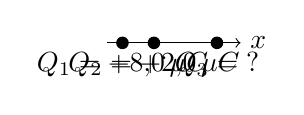
\begin{tikzpicture}[scale=2]
\draw[->] (-0.1,0) -- (0.75,0) node[right] {$x$};
\coordinate (x0) at (0,0);
\coordinate (x1) at (0.2,0);
\coordinate (x2) at (0.6,0);
\fill (x0) circle (0.04) node[below] {$Q_{1}=+8{,}0\,\mu\text{C}$};
\fill (x1) circle (0.04) node[below] {$Q_{2}=+2{,}0\,\mu\text{C}$};
\fill (x2) circle (0.04) node[below] {$Q_{3}=\;?$};
\end{tikzpicture}
\end{center}
%------------------------------------------------------
%------------------------------------------------------
%oefeningen van minstrel
\subsection{oefeningen minstrel}
%------------
% OEF H12
\begin{oef}\label{oH1:H12}
Twee even grote ladingen \( Q_1 \) en \( Q_2 \) bevinden zich op \( 1,00 \, \text{m} \) van elkaar en oefenen op elkaar een kracht uit van \( 1,00 \, \text{N} \). Bepaal de grootte van de ladingen.
\end{oef}
%---------------
%---------------------------
% Oplossing H12
\begin{opl}
\underline{Gegevens:}\\
$\begin{array}{@{}w{l}{0.5\textwidth}@{}}
    F = \qty{1,00}{\newton} \\
    r = \qty{1,00}{\meter} \\
    k = \qty{8,99e9}{\newton\meter\squared\per\coulomb\squared}
\end{array}$

\underline{Gevraagd:} \( Q \) (grootte van de ladingen) \\

\underline{Oplossing:}\\
We gebruiken de \textbf{wet van Coulomb} (vergelijking \ref{eq:coulombkracht}) en lossen op voor \( Q \):

\begin{align*}
    F &= \frac{k \cdot |Q| \cdot |Q|}{r^2} \\
    |Q|^2 &= \frac{F \cdot r^2}{k} \\
    |Q|^2 &= \frac{\qty{1,00}{\newton} \cdot (\qty{1,00}{\meter})^2}{\qty{8,99e9}{\newton\meter\squared\per\coulomb\squared}} \\
    |Q|^2 &= \qty{1,11e-10}{\coulomb\squared} \\
    |Q| &= \sqrt{\qty{1,11e-10}{\coulomb\squared}} \\
    Q &= \pm \qty{1,05e-5}{\coulomb}
\end{align*}

Klik \hyperref[oH1:H12]{hier} om terug naar de vraagstukken te gaan.
\end{opl}
%------------------------------------------------------
%------------
% OEF 2onbekende ladingen
\begin{oef}\label{oH1:2onbekende ladingen}
Twee ladingen op \( 1,00 \, \text{m} \) van elkaar trekken elkaar aan met een kracht van \( 1,00 \, \text{N} \). Hoe groot kunnen die ladingen zijn? Welke van de volgende opties is mogelijk?
a) +1 C en +1 C
b) +1 C en -1 C
c) \( +1,00 \, \mu\text{C} \) en \( -1,1 \cdot 10^{-5} \, \text{C} \)
d) \( +5,6 \cdot 10^{-11} \, \text{C} \) en \( -5,6 \cdot 10^{-11} \, \text{C} \)
\end{oef}
%---------------
%---------------------------
% Oplossing 2onbekende ladingen
\begin{opl}
\underline{Gegevens:}\\
$\begin{array}{@{}w{l}{0.5\textwidth}@{}}
    F = \qty{1,00}{\newton} \\
    r = \qty{1,00}{\meter} \\
    k = \qty{8,99e9}{\newton\meter\squared\per\coulomb\squared}
\end{array}$

\underline{Gevraagd:} Welke optie voldoet aan \( |Q_1| \cdot |Q_2| = \qty{1,11e-10}{\coulomb\squared} \) \\

\underline{Oplossing:}\\
We berekenen het product van de ladingen:

\begin{align*}
    |Q_1| \cdot |Q_2| &= \frac{F \cdot r^2}{k} \\
    &= \frac{\qty{1,00}{\newton} \cdot (\qty{1,00}{\meter})^2}{\qty{8,99e9}{\newton\meter\squared\per\coulomb\squared}} \\
    &= \qty{1,11e-10}{\coulomb\squared}
\end{align*}

Enkel optie c) voldoet: \( |1,00 \cdot 10^{-6} \, \text{C}| \cdot |1,1 \cdot 10^{-5} \, \text{C}| = \qty{1,1e-11}{\coulomb\squared} \)

Klik \hyperref[oH1:2onbekende ladingen]{hier} om terug naar de vraagstukken te gaan.
\end{opl}
%------------------------------------------------------






